%-----------------------------------------------------------------------------------------
% Autor dieser Vorlage:
% Stefan Macke (http://fachinformatiker-anwendungsentwicklung.net)
% Permalink zur Vorlage: http://fiae.link/LaTeXVorlageFIAE
% Lizenz: Creative Commons 4.0 Namensnennung - Weitergabe unter gleichen Bedingungen
% -----------------------------------------------------------------------------------------

\documentclass[
	%ngerman,
	toc=listof, % Abbildungsverzeichnis sowie Tabellenverzeichnis in das Inhaltsverzeichnis aufnehmen
	toc=bibliography, % Literaturverzeichnis in das Inhaltsverzeichnis aufnehmen
	footnotes=multiple, % Trennen von direkt aufeinander folgenden Fußnoten
	parskip=half, % vertikalen Abstand zwischen Absätzen verwenden anstatt horizontale Einrückung von Folgeabsätzen
	numbers=noendperiod, % Den letzten Punkt nach einer Nummerierung entfernen (nach DIN 5008)
	12pt
]{scrartcl}
\pdfminorversion=5 % erlaubt das Einfügen von pdf-Dateien bis Version 1.7, ohne eine Fehlermeldung zu werfen (keine Garantie für fehlerfreies Einbetten!)
\usepackage[utf8]{inputenc} % muss als erstes eingebunden werden, da Meta/Packages ggfs. Sonderzeichen enthalten

% !TEX root = Ausarbeitung.tex

\newcommand{\titel}{Assignment \#2}
\newcommand{\untertitel}{Data Exploration and Preparation}
\newcommand{\kompletterTitel}{\titel{} -- \untertitel}


\newcommand{\betriebLogo}{logo.png}


\newcommand{\betreff}{31250 Introduction to Data Analytics}
 % Metadaten zu diesem Dokument (Autor usw.)
% !TEX root = ../Ausarbeitung.tex

% Anpassung an Landessprache ---------------------------------------------------
\usepackage{babel}
\usepackage{lipsum}
% Umlaute ----------------------------------------------------------------------
%   Umlaute/Sonderzeichen wie äüöß direkt im Quelltext verwenden (CodePage).
%   Erlaubt automatische Trennung von Worten mit Umlauten.
% ------------------------------------------------------------------------------
\usepackage[T1]{fontenc}
\usepackage{textcomp} % Euro-Zeichen etc.
% Schrift ----------------------------------------------------------------------
%\usepackage{lmodern} % bessere Fonts
\usepackage{relsize} % Schriftgröße relativ festlegen

% Tabellen ---------------------------------------------------------------------
\PassOptionsToPackage{table}{xcolor}
\usepackage{tabularx}
% für lange Tabellen
\usepackage{longtable}
\usepackage{array}
\usepackage{ragged2e}
\usepackage{lscape}
\newcolumntype{w}[1]{>{\raggedleft\hspace{0pt}}p{#1}} % Spaltendefinition rechtsbündig mit definierter Breite

% Grafiken ---------------------------------------------------------------------
\usepackage[dvips,final]{graphicx} % Einbinden von JPG-Grafiken ermöglichen
\usepackage{graphics} % keepaspectratio
\usepackage{float} % zum Umfließen von Bildern
\usepackage{wrapfig} % zum Umfließen von Bildern
\graphicspath{{Bilder/}} % hier liegen die Bilder des Dokuments




% Sonstiges --------------------------------------------------------------------
\usepackage[titles]{tocloft} % Inhaltsverzeichnis DIN 5008 gerecht einrücken
\usepackage{amsmath,amsfonts} % Befehle aus AMSTeX für mathematische Symbole
\usepackage{enumitem} % anpassbare Enumerates/Itemizes
\usepackage{xspace} % sorgt dafür, dass Leerzeichen hinter parameterlosen Makros nicht als Makroendezeichen interpretiert werden

\usepackage{makeidx} % für Index-Ausgabe mit \printindex
\usepackage[printonlyused]{acronym} % es werden nur benutzte Definitionen aufgelistet

\usepackage{datetime} % Angabe des Build-Datums auf dem Deckblatt

\usepackage{url}  %url im Literaturverteichnis brechen
\def\UrlBreaks{\do\/\do-}

% Einfache Definition der Zeilenabstände und Seitenränder etc.
\usepackage{setspace}
\usepackage{geometry}

% Symbolverzeichnis
\usepackage[intoc]{nomencl}
\let\abbrev\nomenclature
\renewcommand{\nomname}{Abkürzungsverzeichnis}
\setlength{\nomlabelwidth}{.25\hsize}
\renewcommand{\nomlabel}[1]{#1 \dotfill}
\setlength{\nomitemsep}{-\parsep}

\usepackage{varioref} % Elegantere Verweise. „auf der nächsten Seite“
\usepackage{url} % URL verlinken, lange URLs umbrechen etc.

\usepackage{chngcntr} % fortlaufendes Durchnummerieren der Fußnoten
% \usepackage[perpage]{footmisc} % Alternative: Nummerierung der Fußnoten auf jeder Seite neu

\usepackage{ifthen} % bei der Definition eigener Befehle benötigt
\usepackage{todonotes} % definiert u.a. die Befehle \todo und \listoftodos
\usepackage[square]{natbib} % wichtig für korrekte Zitierweise
\usepackage{float}
% PDF-Optionen -----------------------------------------------------------------
\usepackage{pdfpages}
\pdfminorversion=5 % erlaubt das Einfügen von pdf-Dateien bis Version 1.7, ohne eine Fehlermeldung zu werfen (keine Garantie für fehlerfreies Einbetten!)
\usepackage[
    bookmarks,
    bookmarksnumbered,
    bookmarksopen=true,
    bookmarksopenlevel=1,
    colorlinks=true,
% diese Farbdefinitionen zeichnen Links im PDF farblich aus
    linkcolor=AOBlau, % einfache interne Verknüpfungen
    anchorcolor=AOBlau,% Ankertext
    citecolor=AOBlau, % Verweise auf Literaturverzeichniseinträge im Text
    filecolor=AOBlau, % Verknüpfungen, die lokale Dateien öffnen
    menucolor=AOBlau, % Acrobat-Menüpunkte
    urlcolor=AOBlau,
% diese Farbdefinitionen sollten für den Druck verwendet werden (alles schwarz)
    %linkcolor=black, % einfache interne Verknüpfungen
    %anchorcolor=black, % Ankertext
    %citecolor=black, % Verweise auf Literaturverzeichniseinträge im Text
    %filecolor=black, % Verknüpfungen, die lokale Dateien öffnen
    %menucolor=black, % Acrobat-Menüpunkte
    %urlcolor=black,
%
    %backref, % Quellen werden zurück auf ihre Zitate verlinkt
    pdftex,
    plainpages=false, % zur korrekten Erstellung der Bookmarks
    pdfpagelabels=true, % zur korrekten Erstellung der Bookmarks
    hypertexnames=false, % zur korrekten Erstellung der Bookmarks
    linktocpage % Seitenzahlen anstatt Text im Inhaltsverzeichnis verlinken
]{hyperref}
% Befehle, die Umlaute ausgeben, führen zu Fehlern, wenn sie hyperref als Optionen übergeben werden
\hypersetup{
    pdftitle={\titel -- \untertitel},
    pdfsubject={\titel -- \untertitel},
    pdfkeywords={\titel -- \untertitel},
}


% zum Einbinden von Programmcode -----------------------------------------------
\usepackage{listings}
\usepackage{xcolor}
\definecolor{hellgelb}{rgb}{1,1,0.9}
\definecolor{colKeys}{rgb}{0,0,1}
\definecolor{colIdentifier}{rgb}{0,0,0}
\definecolor{colComments}{rgb}{0,0.5,0}
\definecolor{colString}{rgb}{1,0,0}

\definecolor{lstwhite}{HTML}{000000}
\definecolor{lstblue}{HTML}{0000ff}
\definecolor{lstgreen}{HTML}{a31515}
\definecolor{lstbg}{HTML}{ffffff}

\lstset{
    float=hbp,
	basicstyle=\color{lstwhite},%\ttfamily\footnotesize,
    identifierstyle=\color{lstwhite},
    keywordstyle=\color{lstblue},
    stringstyle=\color{lstgreen},
    commentstyle=\color{lstwhite},
    backgroundcolor=\color{lstbg},
    columns=flexible,
    tabsize=2,
    frame=single,
    extendedchars=true,
    showspaces=false,
    showstringspaces=false,
    numbers=left,
    numberstyle=\footnotesize,
    breaklines=true,
    breakautoindent=true,
	captionpos=b,
    framesep=5pt,
    xleftmargin=0pt,
    xrightmargin=0pt,
}
\lstdefinelanguage{cs}{
    language=[Sharp]C,
    frame=lrb
	sensitive=false,
	morecomment=[l]{//},
	morecomment=[s]{/*}{*/},
	morestring=[b]",
	morekeywords={
		abstract,event,new,struct,as,explicit,null,switch
		base,extern,object,this,bool,false,operator,throw,
		break,finally,out,true,byte,fixed,override,try,
		case,float,params,typeof,catch,for,private,uint,
		char,foreach,protected,ulong,checked,goto,public,unchecked,
		class,if,readonly,unsafe,const,implicit,ref,ushort,
		continue,in,return,using,decimal,int,sbyte,virtual,
		default,interface,sealed,volatile,delegate,internal,short,void,
		do,is,sizeof,while,double,lock,stackalloc,
		else,long,static,enum,namespace,string},
}
\lstdefinelanguage{natural}{
	sensitive=false,
	morecomment=[l]{/*},
	morestring=[b]",
	morestring=[b]',
	alsodigit={-,*},
	morekeywords={
		DEFINE,DATA,LOCAL,END-DEFINE,WRITE,CALLNAT,PARAMETER,USING,
		IF,NOT,END-IF,ON,*ERROR-NR,ERROR,END-ERROR,ESCAPE,ROUTINE,
		PERFORM,SUBROUTINE,END-SUBROUTINE,CONST,END-FOR,END,FOR,RESIZE,
		ARRAY,TO,BY,VALUE,RESET,COMPRESS,INTO,EQ},
}
\lstdefinelanguage{php}{
	sensitive=false,
	morecomment=[l]{/*},
	morestring=[b]",
	morestring=[b]',
	alsodigit={-,*},
	morekeywords={
		abstract,and,array,as,break,case,catch,cfunction,class,clone,const,
		continue,declare,default,do,else,elseif,enddeclare,endfor,endforeach,
		endif,endswitch,endwhile,extends,final,for,foreach,function,global,
		goto,if,implements,interface,instanceof,namespace,new,old_function,or,
		private,protected,public,static,switch,throw,try,use,var,while,xor
		die,echo,empty,exit,eval,include,include_once,isset,list,require,
		require_once,return,print,unset},
}


\lstdefinelanguage{docker}{
    keywords={FROM, RUN, COPY, ADD, ENTRYPOINT, CMD,  ENV, ARG, WORKDIR, EXPOSE, LABEL, USER, VOLUME, STOPSIGNAL, ONBUILD, MAINTAINER},
    keywordstyle=\color{lstblue}\bfseries,
    identifierstyle=\color{lstwhite},
    sensitive=false,
    comment=[l]{\#},
    commentstyle=\color{purple}\ttfamily,
    stringstyle=\color{lstgreen}\ttfamily,
    morestring=[b]',
    morestring=[b]"
}

\lstdefinelanguage{docker-compose}{
    keywords={image, environment, ports, container_name, ports, volumes, links},
    keywordstyle=\color{blue}\bfseries,
    identifierstyle=\color{black},
    sensitive=false,
    comment=[l]{\#},
    commentstyle=\color{purple}\ttfamily,
    stringstyle=\color{red}\ttfamily,
    morestring=[b]',
    morestring=[b]"
}
\lstdefinelanguage{docker-compose-2}{
    keywords={version, volumes, services},
    keywordstyle=\color{blue}\bfseries,
    keywords=[2]{image, environment, ports, container_name, ports, links, build},
    keywordstyle=[2]\color{olive}\bfseries,
    identifierstyle=\color{black},
    sensitive=false,
    comment=[l]{\#},
    commentstyle=\color{purple}\ttfamily,
    stringstyle=\color{red}\ttfamily,
    morestring=[b]',
    morestring=[b]"
}

\lstset{basicstyle=\ttfamily,
    showstringspaces=false,
    commentstyle=\color{red},
    keywordstyle=\color{blue},
    inputencoding=utf8,
    extendedchars=true
} % verwendete Packages
% !TEX root = ../Ausarbeitung.tex

% Seitenränder -----------------------------------------------------------------
\setlength{\topskip}{\ht\strutbox} % behebt Warnung von geometry
\geometry{a4paper,left=25mm,right=25mm,top=30mm,bottom=30mm}

\usepackage[
	automark, % Kapitelangaben in Kopfzeile automatisch erstellen
	headsepline, % Trennlinie unter Kopfzeile
	ilines % Trennlinie linksbündig ausrichten
]{scrpage2}

% Kopf- und Fußzeilen ----------------------------------------------------------
\pagestyle{scrheadings}
% chapterpagestyle gibt es nicht in scrartcl
%\renewcommand{\chapterpagestyle}{scrheadings}
\clearscrheadfoot

% Kopfzeile
\renewcommand{\headfont}{\normalfont} % Schriftform der Kopfzeile
\ihead{\textsc{\titel}\\[0.5ex] \textit{\headmark}}
\chead{}
\ohead{\includegraphics[scale=0.25]{\betriebLogo}}
\setlength{\headheight}{15mm} % Höhe der Kopfzeile
%\setheadwidth[0pt]{textwithmarginpar} % Kopfzeile über den Text hinaus verbreitern (falls Logo den Text überdeckt)

% Fußzeile
\ifoot{\today}
\cfoot{}
\ofoot{\pagemark}
\setlength{\footskip}{10mm}

% Überschriften nach DIN 5008 in einer Fluchtlinie
% ------------------------------------------------------------------------------

% Abstand zwischen Nummerierung und Überschrift definieren
% > Schön wäre hier die dynamische Berechnung des Abstandes in Abhängigkeit
% > der Verschachtelungstiefe des Inhaltsverzeichnisses
\newcommand{\headingSpace}{1.5cm}

% Abschnittsüberschriften im selben Stil wie beim Inhaltsverzeichnis einrücken
\renewcommand*{\othersectionlevelsformat}[3]{
  \makebox[\headingSpace][l]{#3\autodot}
}

% Für die Einrückung wird das Paket tocloft benötigt
%\cftsetindents{chapter}{0.0cm}{\headingSpace}
\cftsetindents{section}{0.0cm}{\headingSpace}
\cftsetindents{subsection}{0.0cm}{\headingSpace}
\cftsetindents{subsubsection}{0.0cm}{\headingSpace}
\cftsetindents{figure}{0.0cm}{\headingSpace}
\cftsetindents{table}{0.0cm}{\headingSpace}


% Allgemeines
% ------------------------------------------------------------------------------

%\onehalfspacing % Zeilenabstand 1,5 Zeilen
\frenchspacing % erzeugt ein wenig mehr Platz hinter einem Punkt

% Schusterjungen und Hurenkinder vermeiden
\clubpenalty = 10000
\widowpenalty = 10000
\displaywidowpenalty = 10000

% Quellcode-Ausgabe formatieren
%\lstset{numbers=left, numberstyle=\tiny, numbersep=5pt, breaklines=true}
\lstset{emph={square}, emphstyle=\color{red}, emph={[2]root,base}, emphstyle={[2]\color{blue}}}

\counterwithout{footnote}{section} % Fußnoten fortlaufend durchnummerieren
\setcounter{tocdepth}{\subsubsectionlevel} % im Inhaltsverzeichnis werden die Kapitel bis zum Level der subsubsection übernommen
\setcounter{secnumdepth}{\subsubsectionlevel} % Kapitel bis zum Level der subsubsection werden nummeriert

% Aufzählungen anpassen
\renewcommand{\labelenumi}{\arabic{enumi}.}
\renewcommand{\labelenumii}{\arabic{enumi}.\arabic{enumii}.}
\renewcommand{\labelenumiii}{\arabic{enumi}.\arabic{enumii}.\arabic{enumiii}}

% Tabellenfärbung:
\definecolor{heading}{rgb}{0.64,0.78,0.86}
\definecolor{odd}{rgb}{0.9,0.9,0.9}

% Schriftart
\usepackage[sfdefault, scale=1, light]{roboto}  % Roboto als Schrifart
\usepackage[T1]{fontenc}
\usepackage{newtxsf}
 % Definitionen zum Aussehen der Seiten
% Tabellen, die den Zwischenstand nach einer Projektphase verdeutlichen
\newcommand{\Zwischenstand}[2]{\subsection{Zwischenstand}Tabelle~\ref{tab:#2} zeigt den Zwischenstand nach der #1.\tabelle{Zwischenstand nach der #1}{tab:#2}{#2.tex}}

% Abkürzungen
\newcommand{\Versis}{\textsc{Versis}\xspace}
\newcommand{\NI}{NatInfo\xspace}

\newcommand{\FVS}{Ferdinand-von-Steinbeisschule Reutlingen\xspace}


%Todo

\newcommand{\TODO}[1]{\textbf{\LARGE\color{red} #1}}
\newcommand{\code}[1]{\texttt{#1}} % eigene allgemeine Befehle, die z.B. die Arbeit mit LaTeX erleichtern
% Tabellen, die den Zwischenstand nach einer Projektphase verdeutlichen
\newcommand{\Zwischenstand}[2]{\subsection{Zwischenstand}Tabelle~\ref{tab:#2} zeigt den Zwischenstand nach der #1.\tabelle{Zwischenstand nach der #1}{tab:#2}{#2.tex}}

% Abkürzungen
\newcommand{\Versis}{\textsc{Versis}\xspace}
\newcommand{\NI}{NatInfo\xspace}

\newcommand{\FVS}{Ferdinand-von-Steinbeisschule Reutlingen\xspace}


%Todo

\newcommand{\TODO}[1]{\textbf{\LARGE\color{red} #1}}
\newcommand{\code}[1]{\texttt{#1}} % eigene projektspezifische Befehle, z.B. Abkürzungen usw.

\begin{document}


\phantomsection
\thispagestyle{plain}
\pdfbookmark[1]{Deckblatt}{deckblatt}
% !TEX root = Ausarbeitung.tex
\begin{titlepage}

\begin{center}

\includegraphics[scale=0.8]{logo.png}\\[5ex]


\large{\betreff}\\[3.5ex]

\LARGE{\textbf{\titel}}\\[1.5ex]
\large{\untertitel}\\[3.5ex]

\normalsize

\begin{tabular}{c}

\end{tabular}

\textbf{\Large{Florian Lubitz}}\\
FEIT\\
13688799\\
florian.lubitz@student.uts.edu.au
\\[3ex]

\end{center}

\end{titlepage}
\cleardoublepage

% Preface --------------------------------------------------------------------
\phantomsection
\pagenumbering{gobble}
%\pagenumbering{arabic}
\setcounter{tocdepth}{2}
\pdfbookmark[1]{Inhaltsverzeichnis}{inhalt}
\tableofcontents
\cleardoublepage


\pagenumbering{arabic}
% Inhalt ---------------------------------------------------------------------
% !TeX spellcheck = en_US
% !TEX root = Ausarbeitung.tex

\section{Initial data exploration}
\subsection{Attribute features}
\subsubsection{Quote\_Id}
\paragraph{Attribute type: nominal}
The "Quote\_Id" is a customer number. It is neither orderable nor is the number a quantitative value. As the id is a unique key, there is no reason to perform any statistic analysis on this attribute.


\subsubsection{Quote\_Date}
\paragraph{Attribute type: interval}
"Quote\_Date" seems to be a date. These have a fixed sequence and plus and minus operations can be performed with them.
 
\begin{table}[H]
	\renewcommand{\arraystretch}{1.25}
	\begin{tabular}{l|l}
		\textbf{Statistic} & \textbf{Value}\\\hline
		Missing Values& None\\\hline
		Minimum& 02.01.2013\\\hline
		Maximum& 18.05.2015\\\hline
		Mean& 23.03.2014\\\hline
		Std. Dev.& $245$ d\\\hline
	\end{tabular}
\end{table}

\begin{figure}[H]
	\begin{center}
		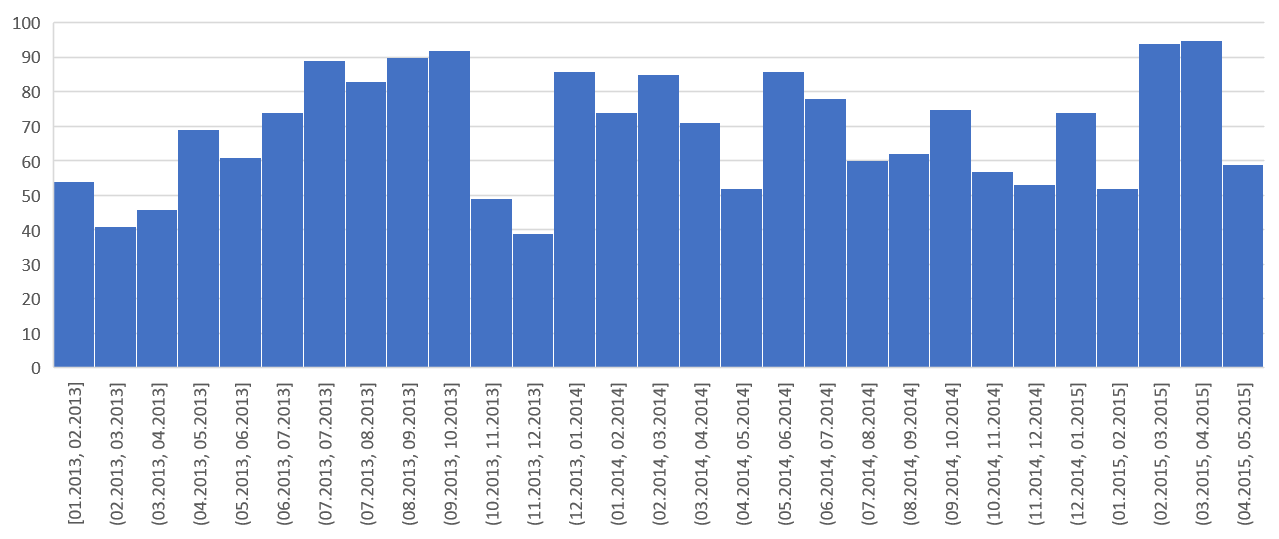
\includegraphics[width=0.8\textwidth]{Histo_Quote_Date.png}
	\end{center}
	\caption{Histogramm Quote\_Date}
\end{figure}


\subsubsection{Quote\_Flag}
\paragraph{Attribute type: nominal (dichotomous)}
The description of the attributes declares "Quote\_Flag" as information about whether an insurance was purchased. This can be only answered with yes or no.

\begin{table}[H]
	\renewcommand{\arraystretch}{1.25}
	\begin{tabular}{l|l}
		\textbf{Statistic} & \textbf{Value}\\\hline
		Missing Values& None\\\hline
	\end{tabular}
\end{table}

\begin{table}[H]
	\renewcommand{\arraystretch}{1.25}
		\begin{tabular}{l|l|l}
			\textbf{Value} & \textbf{Absolute Frequency} & \textbf{Relative Frequency}\\\hline
			0 & $1605$ & $0.8025$\\ \hline
			1 & $395$ & $0.1975$\\
		\end{tabular}
\end{table}

\begin{figure}[H]
	\begin{center}
		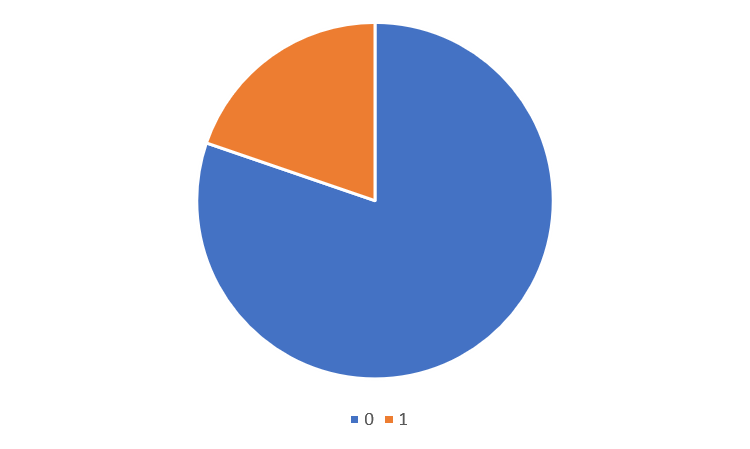
\includegraphics[width=0.8\textwidth]{Pie_Quote_Flag.png}
	\end{center}
	\caption{Pie Graph Quote\_Flag}
\end{figure}


\subsubsection{Field\_Info1}
\paragraph{Attribute type: nominal} These characters are not close enough together to asssume, they belong to a ordererd attribute.

\begin{table}[H]
	\renewcommand{\arraystretch}{1.25}
	\begin{tabular}{l|l}
		\textbf{Statistic} & \textbf{Value}\\\hline
		Missing Values& None\\\hline
	\end{tabular}
\end{table}


\begin{table}[H]
	\renewcommand{\arraystretch}{1.25}
	\begin{tabular}{l|l|l}
		\textbf{Value} & \textbf{Absolute Frequency} & \textbf{Relative Frequency}\\\hline
			J&$390$ & $0.365$\\\hline
			F&$540$ & $0.27$\\\hline
			B&$730$ & $0.195$\\\hline
			E&$200$ & $0.1$\\\hline
			C&$39$ & $0.0505$\\\hline
			K&$101$ & $0.0195$\\
	\end{tabular}
\end{table}

\begin{figure}[H]
	\begin{center}
		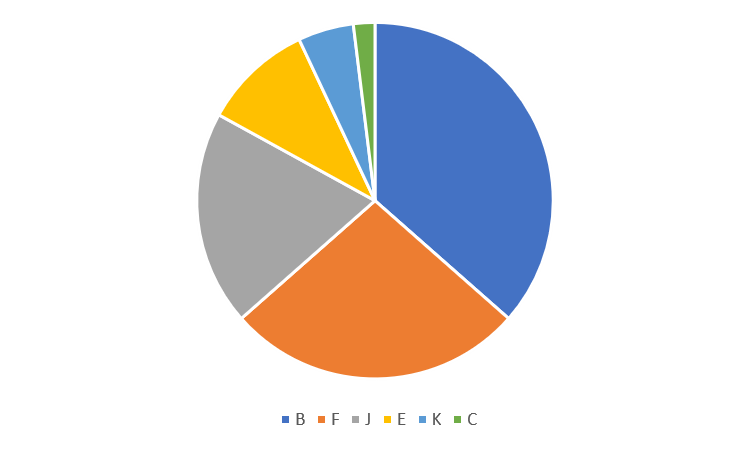
\includegraphics[width=0.8\textwidth]{Pie_Field_Info2.png}
	\end{center}
	\caption{Pie Graph Field\_Info1}
\end{figure}


\subsubsection{Field\_Info2}
\paragraph{Attribute type: ratio}
All values of "Field\_Info2" are numbers between $0$ and $2$ and have a precision of 4 decimals. This suggests that these values are on a zero-based scale.
\begin{table}[H]
	\renewcommand{\arraystretch}{1.25}
	\begin{tabular}{l|l}
		\textbf{Statistic} & \textbf{Value}\\\hline
			Missing Values& None\\\hline
			Minimum& $0.8746$\\\hline
			Maximum& $1.0101$\\\hline
			Mean& $0.9391$\\\hline
			Std. Dev.& $0.0373$\\\hline
			90th Perc. & $1.00051$\\\hline
			10th Perc. & $0.8922$ \\
	\end{tabular}
\end{table}

\begin{figure}[H]
	\begin{center}
		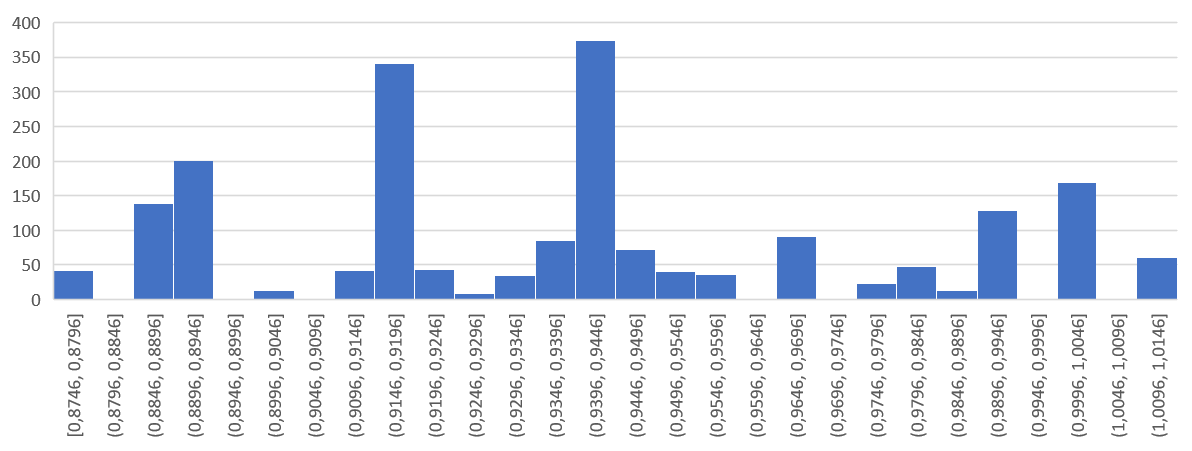
\includegraphics[width=0.8\textwidth]{Histo_Field_Info2.png}
	\end{center}
	\caption{Histogramm Field\_Info2}
\end{figure}

\subsubsection{Field\_Info3}
\paragraph{Attribute type: ratio} The values in this attribute are all numeric range in a range of around $1000$. Given the size of the numbers this could be a attribute containing monetary values.

\begin{table}[H]
	\renewcommand{\arraystretch}{1.25}
	\begin{tabular}{l|l}
		\textbf{Statistic} & \textbf{Value}\\\hline
			Missing Values& None\\\hline
		Minimum& $548$\\\hline
		Maximum& $1487$\\\hline
		Mean& $950.5195$\\\hline
		Std. Dev.& $290.62$\\\hline
		90th Perc. & $901480$\\\hline
		10th Perc. & $548$ \\		
	\end{tabular}
\end{table}

\begin{figure}[H]
	\begin{center}
		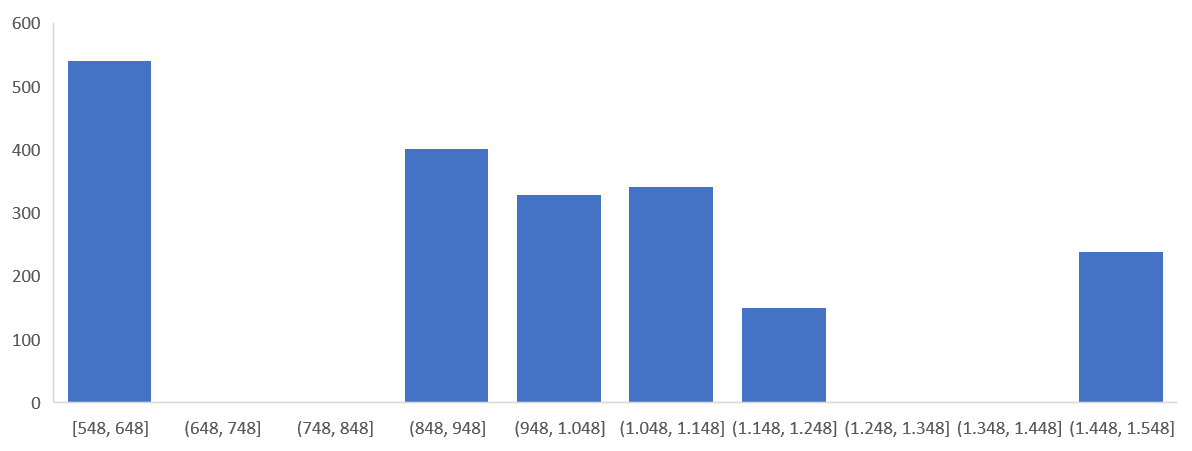
\includegraphics[width=0.8\textwidth]{Histo_Field_Info3.png}
	\end{center}
	\caption{Histogramm Field\_Info3}
\end{figure}

\subsubsection{Field\_Info4}
\paragraph{Attribute type: nominal (dichotomous)} In this Attribute only the values "Y" and "N" appear. Those values are often used as a short version on "Yes" and "No". This field therefore seems to be a yes-no answer.
\qquad
\begin{table}[H]
	\renewcommand{\arraystretch}{1.25}
	\begin{tabular}{l|l}
		\textbf{Statistic} & \textbf{Value}\\\hline
		Missing Values& None\\\hline
	\end{tabular}
\end{table}
\begin{table}[H]
	\renewcommand{\arraystretch}{1.25}
	\begin{tabular}{l|l|l}
		\textbf{Value} & \textbf{Absolute Frequency} & \textbf{Relative Frequency}\\\hline
		N	&$1860$&$0.93$\\\hline
		Y&	$140$&$0.07$
	\end{tabular}
\end{table}

\begin{figure}[H]
	\begin{center}
		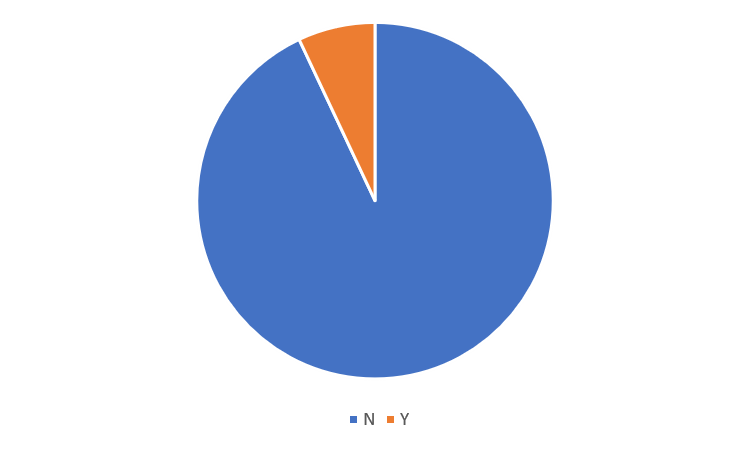
\includegraphics[width=0.8\textwidth]{Pie_Field_Info4.png}
	\end{center}
	\caption{Pie Graph Field\_Info4}
\end{figure}

\subsubsection{Coverage\_Info1}
\paragraph{Attribute type: ordinal} This attribute contains values from $1$ to $25$.  These could be different values in a specified order but not a numeric value.

\begin{table}[H]
	\renewcommand{\arraystretch}{1.25}
	\begin{tabular}{l|l}
		\textbf{Statistic} & \textbf{Value}\\\hline
		Missing Values& None\\\hline
		Numeric Outliers & $74$
	\end{tabular}
\end{table}

\begin{table}[H]
	\renewcommand{\arraystretch}{1.25}
	\begin{tabular}{l|l|l}
		\textbf{Value} & \textbf{Absolute Frequency} & \textbf{Relative Frequency}\\\hline
		-1&$2$&$0.001$\\\hline
		1&$42$&$0.021$\\\hline
		2&$81$&$0.0405$\\\hline
		3&$118$&$0.059$\\\hline
		4&$149$&$0.0745$\\\hline
		5&$189$&$0.0945$\\\hline
		6&$182$&$0.091$\\\hline
		7&$185$&$0.0925$\\\hline
		8&$148$&$0.074$\\\hline
		9&$151$&$0.0755$\\\hline
		10&$113$&$0.0565$\\\hline
		11&$106$&$0.053$\\\hline
		12&$83$&$0.0415$\\\hline
		13&$67$&$0.0335$\\\hline
		14&$62$&$0.031$\\\hline
		15&$53$&$0.0265$\\\hline
		16&$49$&$0.0245$\\\hline
		17&$35$&$0.0175$\\\hline
		18&$37$&$0.0185$\\\hline
		19&$19$&$0.0095$\\\hline
		20&$18$&$0.009$\\\hline
		21&$19$&$0.0095$\\\hline
		22&$18$&$0.009$\\\hline
		23&$12$&$0.006$\\\hline
		24&$11$&$0.0055$\\\hline
		25&$51$&$0.0255$
	\end{tabular}
\end{table}

\begin{figure}[H]
	\begin{center}
		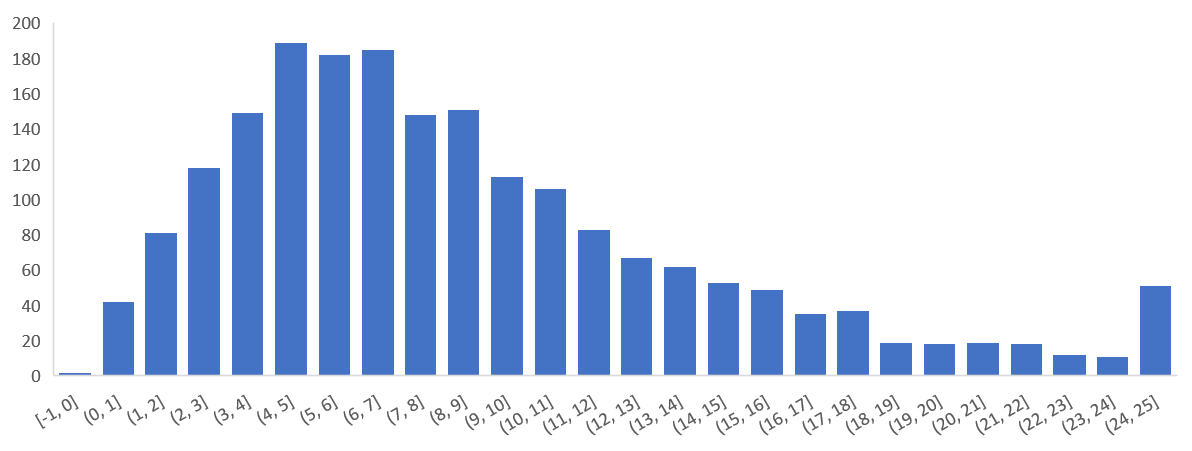
\includegraphics[width=0.8\textwidth]{Histo_Coverage_Info1.png}
	\end{center}
	\caption{Histogramm Coverage\_Info1}
\end{figure}

\subsubsection{Coverage\_Info2}
\paragraph{Attribute type: ordinal}As before, this attribute contains values from $1$ to $25$.  These could be different values in a specified order but not a numeric value but we only got datapoints with values at $1$,$2$, $22$ and $25$, which is quite interesting as only $3$ customers selected value $1$

\begin{table}[H]
	\renewcommand{\arraystretch}{1.25}
	\begin{tabular}{l|l}
		\textbf{Statistic} & \textbf{Value}\\\hline
		Missing Values& None\\\hline
	\end{tabular}
\end{table}
\begin{table}[H]
	\renewcommand{\arraystretch}{1.25}
	\begin{tabular}{l|l|l}
		\textbf{Value} & \textbf{Absolute Frequency} & \textbf{Relative Frequency}\\\hline
		1&$3$&$0.0015$\\\hline
		2&$125$&$0.0625$\\\hline
		22&$1620$&$0.81$\\\hline
		25&$252$&$0.126$\\\hline
	\end{tabular}
\end{table}

\begin{figure}[H]
	\begin{center}
		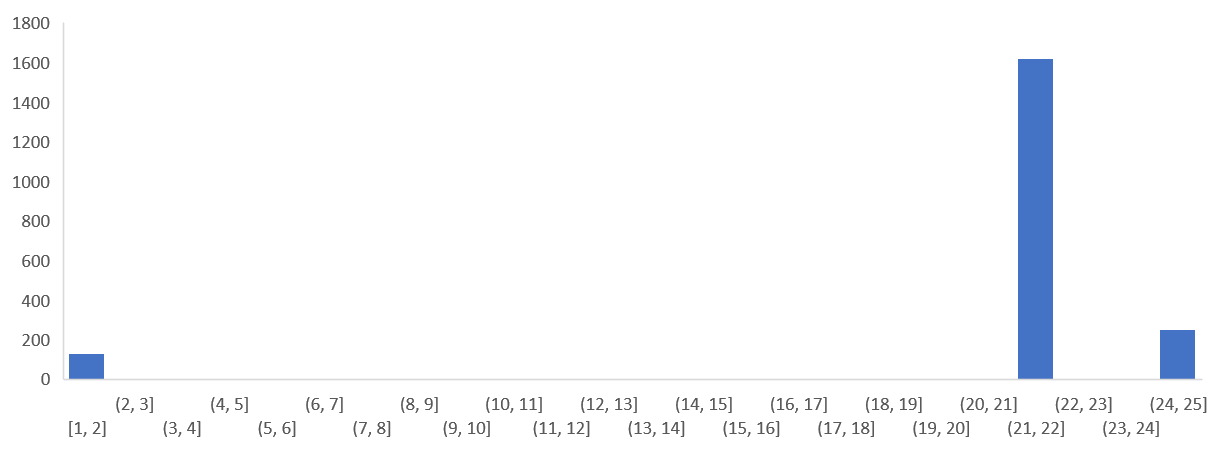
\includegraphics[width=0.8\textwidth]{Histo_Coverage_Info2.png}
	\end{center}
	\caption{Histogramm Coverage\_Info2}
\end{figure}

\subsubsection{Coverage\_Info3}
\paragraph{Attribute type: ordinal} This field contains letters from the beginning of the alphabet. This indicates for these values to be ordered in that order.

\begin{table}[H]
	\renewcommand{\arraystretch}{1.25}
	\begin{tabular}{l|l}
		\textbf{Statistic} & \textbf{Value}\\\hline
		Missing Values& None\\\hline
	\end{tabular}
\end{table}
\begin{table}[H]
	\renewcommand{\arraystretch}{1.25}
	\begin{tabular}{l|l|l}
		\textbf{Value} & \textbf{Absolute Frequency} & \textbf{Relative Frequency}\\\hline
		A&$116$&$0.058$\\\hline
		B&$4$&$0.002$\\\hline
		C&$3$&$0.0015$\\\hline
		D&$388$&$0.194$\\\hline
		E&$673$&$0.3365$\\\hline
		F&$221$&$0.1105$\\\hline
		G&$245$&$0.1225$\\\hline
		H&$2$&$0.001$\\\hline
		I&$7$&$0.0035$\\\hline
		J&$110$&$0.055$\\\hline
		K&$229$&$0.1145$\\\hline
		L&$2$&$0.001$
	\end{tabular}
\end{table}
\begin{figure}[H]
	\begin{center}
		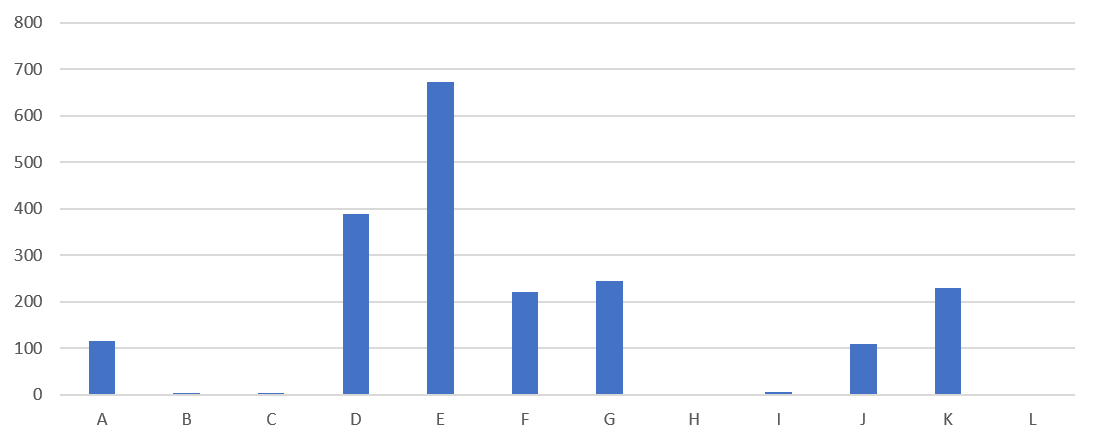
\includegraphics[width=0.8\textwidth]{Histo_Coverage_Info3.png}
	\end{center}
	\caption{Histogramm Coverage\_Info3}
\end{figure}

\pagebreak
\subsubsection{Sales\_Info1}
\paragraph{Attribute type: nominal (dichotomous)}
\qquad
\begin{table}[H]
	\renewcommand{\arraystretch}{1.25}
	\begin{tabular}{l|l}
		\textbf{Statistic} & \textbf{Value}\\\hline
		Missing Values& None\\\hline
	\end{tabular}
\end{table}
\begin{table}[H]
	\renewcommand{\arraystretch}{1.25}
	\begin{tabular}{l|l|l}
		\textbf{Value} & \textbf{Absolute Frequency} & \textbf{Relative Frequency}\\\hline
		1&$1490$&$0.745$\\\hline
		0&$510$&$0.255$
	\end{tabular}
\end{table}
\begin{figure}[H]
	\begin{center}
		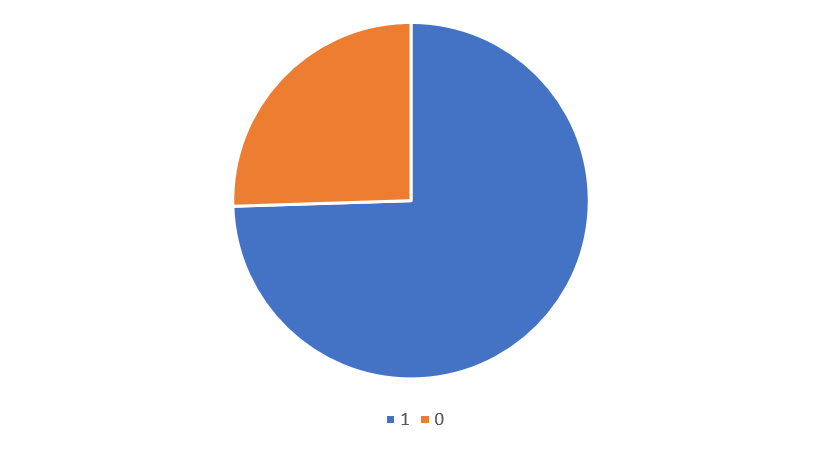
\includegraphics[width=0.8\textwidth]{Pie_Sales_Info1.png}
	\end{center}
	\caption{Pie Graph Sales\_Info1}
\end{figure}

\subsubsection{Sales\_Info2}
\paragraph{Attribute type: ordinal} This Attributes contains numbers from $2$ to $5$. Probably, the provided data is missing the value $1$. With that value these could be values ordered from $1$ to $5$.
\qquad
\begin{table}[H]
	\renewcommand{\arraystretch}{1.25}
	\begin{tabular}{l|l}
		\textbf{Statistic} & \textbf{Value}\\\hline
		Missing Values& None\\\hline
	\end{tabular}
\end{table}
\begin{table}[H]
	\renewcommand{\arraystretch}{1.25}
	\begin{tabular}{l|l|l}
		\textbf{Value} & \textbf{Absolute Frequency} & \textbf{Relative Frequency}\\\hline
		2&$93$&$0.0465$\\\hline
		3&$519$&$0.2595$\\\hline
		4&$295$&$0.1475$\\\hline
		5&$1093$&$0.5465$
	\end{tabular}
\end{table}
\begin{figure}[H]
	\begin{center}
		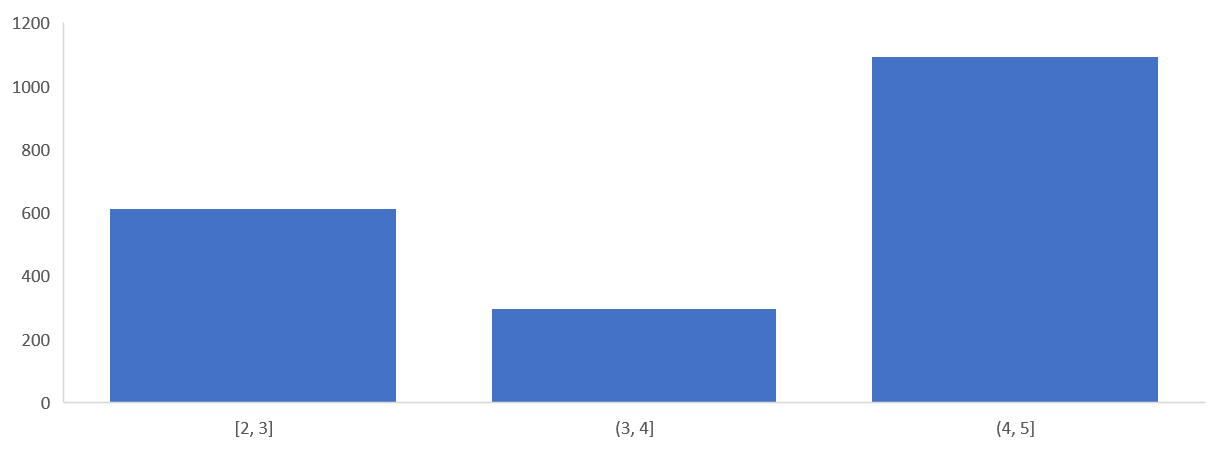
\includegraphics[width=0.8\textwidth]{Histo_Sales_Info2.png}
	\end{center}
	\caption{Histogramm Sales\_Info2}
\end{figure}

\subsubsection{Sales\_Info3}
\paragraph{Attribute type: ordinal} Like Coverage\_Info1 this is a ordinal attribute, but we are missing some values inside the provided range.

\qquad
\begin{table}[H]
	\renewcommand{\arraystretch}{1.25}
	\begin{tabular}{l|l}
		\textbf{Statistic} & \textbf{Value}\\\hline
		Missing Values& None\\\hline
	\end{tabular}
\end{table}
\begin{figure}[H]
	\begin{center}
		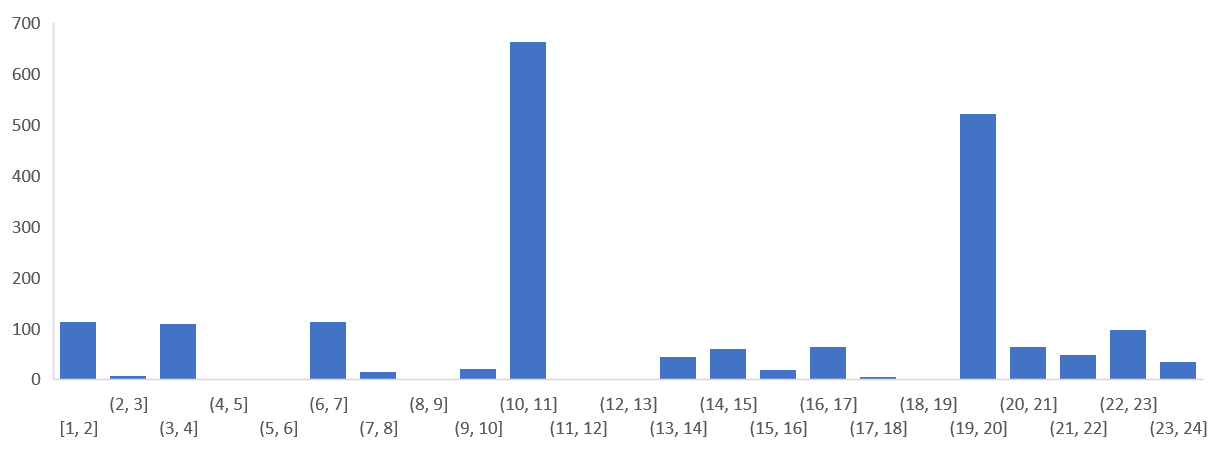
\includegraphics[width=0.8\textwidth]{Histo_Sales_Info3.png}
	\end{center}
	\caption{Histogramm Sales\_Info3}
\end{figure}

\subsubsection{Sales\_Info4}
\paragraph{Attribute type: nominal} These letters seem to have no recognisable order.

\begin{table}[H]
	\renewcommand{\arraystretch}{1.25}
	\begin{tabular}{l|l}
		\textbf{Statistic} & \textbf{Value}\\\hline
		Missing Values& None\\\hline
	\end{tabular}
\end{table}
\begin{table}[H]
	\renewcommand{\arraystretch}{1.25}
	\begin{tabular}{l|l|l}
		\textbf{Value} & \textbf{Absolute Frequency} & \textbf{Relative Frequency}\\\hline
		K&$410$&$0.205$\\\hline
		P&$376$&$0.188$\\\hline
		T&$332$&$0.166$\\\hline
		Q&$312$&$0.156$\\\hline
		V&$298$&$0.149$\\\hline
		R&$156$&$0.078$\\\hline
		M&$116$&$0.058$
	\end{tabular}
\end{table}

\begin{figure}[H]
	\begin{center}
		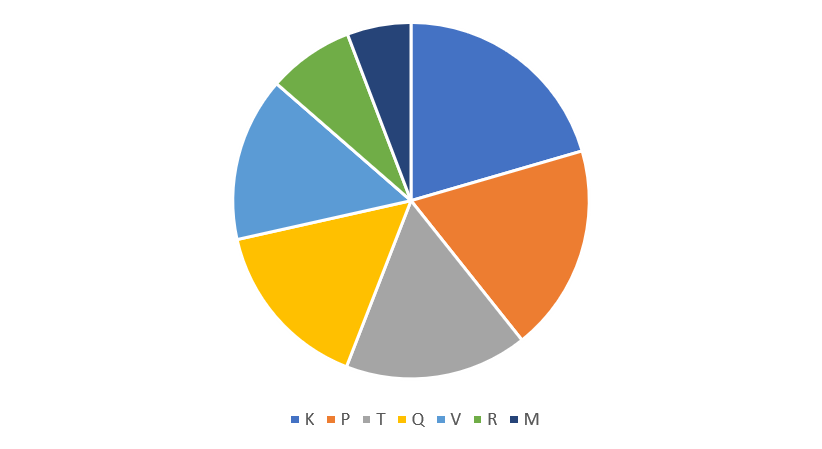
\includegraphics[width=0.8\textwidth]{Pie_Sales_Info4.png}
	\end{center}
	\caption{Pie Graph Sales\_Info4}
\end{figure}

\subsubsection{Sales\_Info5}
\paragraph{Attribute type: ratio} The values in this attribute are distributed very evenly and range in a big range. Given the size of the numbers this could be a attribute containing monetary values.

\begin{table}[H]
	\renewcommand{\arraystretch}{1.25}
	\begin{tabular}{l|l}
		\textbf{Statistic} & \textbf{Value}\\\hline
		Missing Values& None\\\hline
		Minimum& $1$\\\hline
		Maximum& $67162$\\\hline
		Mean& $33785.54$\\\hline
		Std. Dev.& $18863.43$\\\hline
		90th Perc. & $59741.7$\\\hline
		10th Perc. & $7828.9$ \\		
	\end{tabular}
\end{table}
\begin{figure}[H]
	\begin{center}
		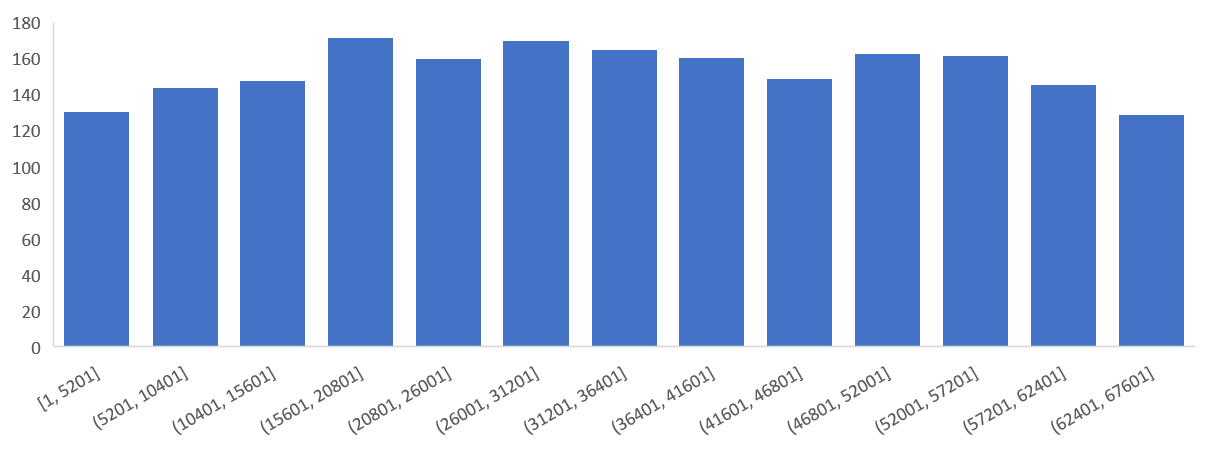
\includegraphics[width=0.8\textwidth]{Histo_Sales_Info5.png}
	\end{center}
	\caption{Histogramm Sales\_Info5}
\end{figure}

\subsubsection{Personal\_Info1}
\paragraph{Attribute type: nominal (dichotomous)}\quad

\begin{table}[H]
	\renewcommand{\arraystretch}{1.25}
	\begin{tabular}{l|l}
		\textbf{Statistic} & \textbf{Value}\\\hline
		Missing Values& None\\\hline
	\end{tabular}
\end{table}
\begin{table}[H]
	\renewcommand{\arraystretch}{1.25}
	\begin{tabular}{l|l|l}
		\textbf{Value} & \textbf{Absolute Frequency} & \textbf{Relative Frequency}\\\hline
		N&$1993$&$0.9965$\\\hline
		Y&$7$&$0.0035$
	\end{tabular}
\end{table}

\begin{figure}[H]
	\begin{center}
		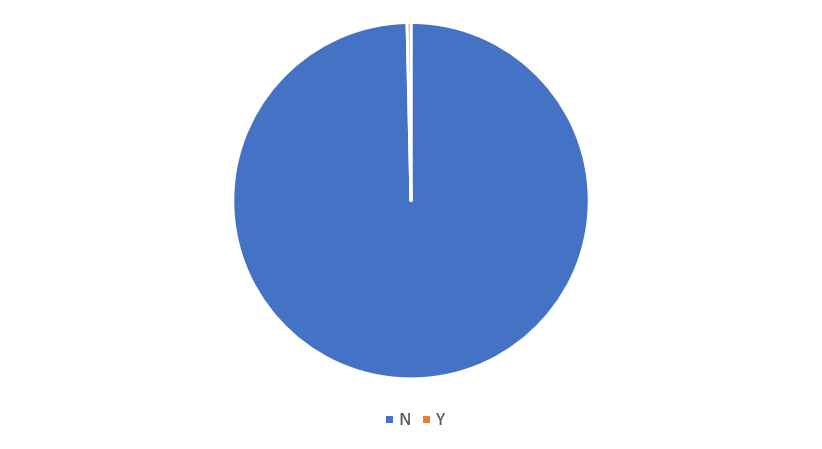
\includegraphics[width=0.8\textwidth]{Pie_Personal_Info1.png}
	\end{center}
	\caption{Pie Graph Personal\_Info1}
\end{figure}

\subsubsection{Personal\_Info2}
\paragraph{Attribute type: ordinal} Like Coverage\_Info1, this attribute probably also contains ordered values, but in the range between $1$ and $25$. And the value $-1$ means "no answer". 

\begin{table}[H]
	\renewcommand{\arraystretch}{1.25}
	\begin{tabular}{l|l}
		\textbf{Statistic} & \textbf{Value}\\\hline
		Missing Values& None\\\hline
	\end{tabular}
\end{table}
\begin{figure}[H]
	\begin{center}
		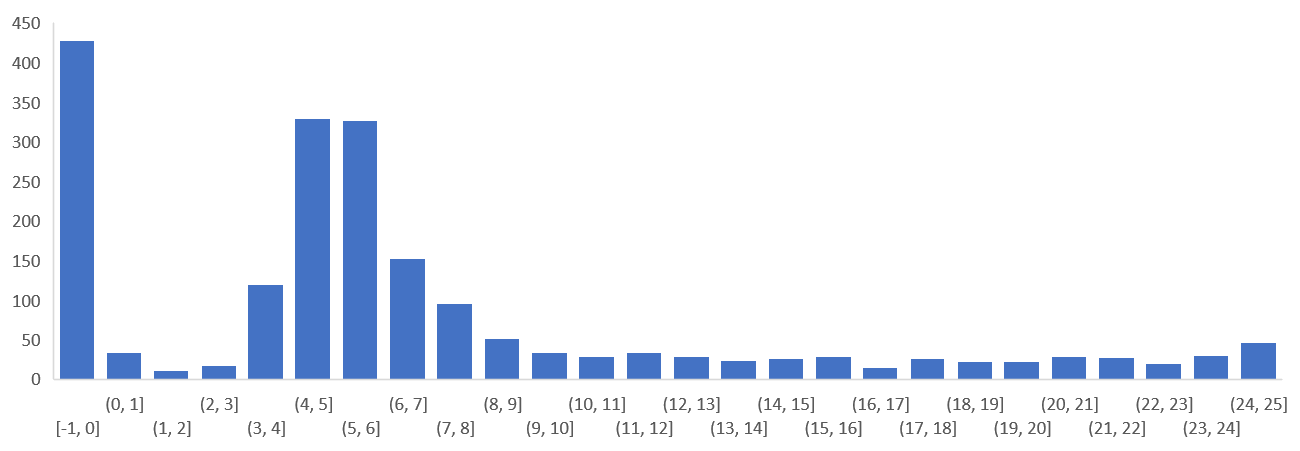
\includegraphics[width=0.8\textwidth]{Histo_Personal_Info2.png}
	\end{center}
	\caption{Histogramm Personal\_Info2}
\end{figure}

\subsubsection{Personal\_Info3}
\paragraph{Attribute type: nominal} These two letter combinations could be order in a alphabetic order, but they seem to start at a random place inside the alphabet. Therefore this attribute will be treated as nominal.

\begin{table}[H]
	\renewcommand{\arraystretch}{1.25}
	\begin{tabular}{l|l}
		\textbf{Statistic} & \textbf{Value}\\\hline
		Missing Values& None\\\hline
	\end{tabular}
\end{table}
\begin{table}[H]
	\renewcommand{\arraystretch}{1.25}
	\begin{tabular}{l|l|l}
		\textbf{Value} & \textbf{Absolute Frequency} & \textbf{Relative Frequency}\\\hline
		ZA&$937$&$0.4685$\\\hline
		XR&$104$&$0.052$\\\hline
		XM&$81$&$0.0405$\\\hline
		XJ&$73$&$0.0365$\\\hline
		XD&$63$&$0.0315$\\\hline
		XX&$62$&$0.031$\\\hline
		XB&$59$&$0.0295$\\\hline
		YH&$58$&$0.029$\\\hline
		XH&$54$&$0.027$\\\hline
		ZT&$51$&$0.0255$\\\hline
		XO&$50$&$0.025$\\\hline
		ZF&$46$&$0.023$\\\hline
		ZR&$40$&$0.02$\\\hline
		ZN&$39$&$0.0195$\\\hline
		ZH&$37$&$0.0185$\\\hline
		XS&$35$&$0.0175$\\\hline
		YF&$29$&$0.0145$\\\hline
		XW&$23$&$0.0115$\\\hline
		ZG&$20$&$0.01$\\\hline
		XE&$20$&$0.01$\\\hline
		ZW&$18$&$0.009$\\\hline
		YE&$17$&$0.0085$\\\hline
		ZC&$16$&$0.008$\\\hline
		XC&$14$&$0.007$\\\hline
		XQ&$14$&$0.007$\\\hline
		XL&$7$&$0.0035$\\\hline
		ZE&$7$&$0.0035$\\\hline
		ZJ&$6$&$0.003$\\\hline
		XI&$5$&$0.0025$\\\hline
		ZD&$5$&$0.0025$\\\hline
		ZK&$4$&$0.002$\\\hline
		XZ&$4$&$0.002$\\\hline
		ZU&$2$&$0.001$
	\end{tabular}
\end{table}

\begin{figure}[H]
	\begin{center}
		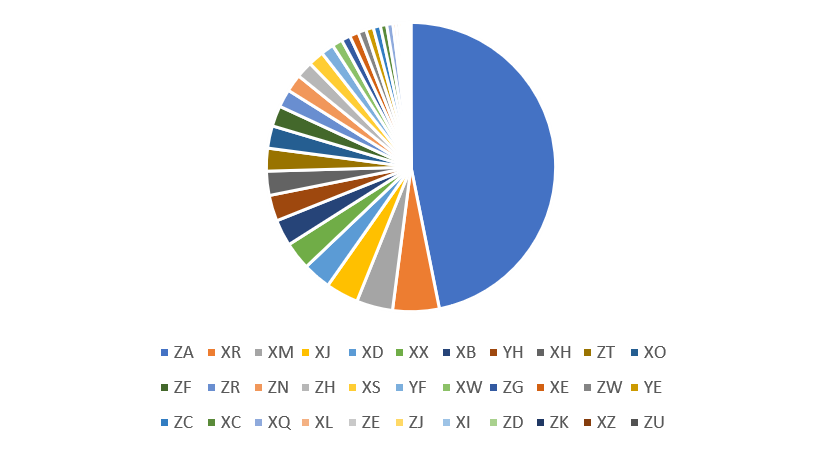
\includegraphics[width=0.8\textwidth]{Pie_Personal_Info3.png}
	\end{center}
	\caption{Pie Graph Personal\_Info3}
\end{figure}

\subsubsection{Personal\_Info4}
\paragraph{Attribute type: nominal (dichotomous)} \quad All those values are $0$ except for one, which is $1$.

\begin{table}[H]
	\renewcommand{\arraystretch}{1.25}
	\begin{tabular}{l|l}
		\textbf{Statistic} & \textbf{Value}\\\hline
		Missing Values& None\\\hline
		Outliers & $1$
	\end{tabular}
\end{table}
\begin{table}[H]
	\renewcommand{\arraystretch}{1.25}
	\begin{tabular}{l|l|l}
		\textbf{Value} & \textbf{Absolute Frequency} & \textbf{Relative Frequency}\\\hline
		0&$1999$&$0.9995$\\\hline
		1&$1$&$0.001$
	\end{tabular}
\end{table}


\subsubsection{Personal\_Info5}
\paragraph{Attribute type: ordinal}This Attribute has no value in a lot of Cases. This Attribute could have up to 5 different, ordered values ($1$ - $5$). This Attribute will probably not get looked at during prediction analysis.

\begin{table}[H]
	\renewcommand{\arraystretch}{1.25}
	\begin{tabular}{l|l}
		\textbf{Statistic} & \textbf{Value}\\\hline
		Missing Values& $966$\\\hline
	\end{tabular}
\end{table}

\subsubsection{Property\_Info1}
\paragraph{Attribute type: nominal (dichotomous)}
\begin{table}[H]
	\renewcommand{\arraystretch}{1.25}
	\begin{tabular}{l|l}
		\textbf{Statistic} & \textbf{Value}\\\hline
		Missing Values& $1$\\\hline
	\end{tabular}
\end{table}
\begin{table}[H]
	\renewcommand{\arraystretch}{1.25}
	\begin{tabular}{l|l|l}
		\textbf{Value} & \textbf{Absolute Frequency} & \textbf{Relative Frequency}\\\hline
		N&$1738$&$0.869$\\\hline
		Y&$261$&$0.1305$
\end{tabular}
\end{table}

\begin{figure}[H]
	\begin{center}
		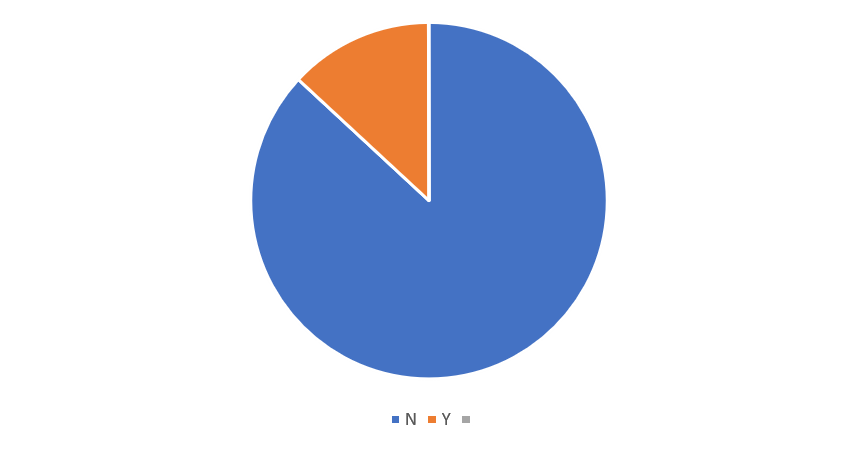
\includegraphics[width=0.8\textwidth]{Pie_Property_Info1.png}
	\end{center}
	\caption{Pie Graph Property\_Info1}
\end{figure}

\subsubsection{Property\_Info2}
\paragraph{Attribute type: nominal} All those values are $0$

\begin{table}[H]
	\renewcommand{\arraystretch}{1.25}
	\begin{tabular}{l|l}
		\textbf{Statistic} & \textbf{Value}\\\hline
		Missing Values& None\\\hline
	\end{tabular}
\end{table}


\subsubsection{Property\_Info3}
\paragraph{Attribute type: nominal} random letters

\begin{table}[H]
	\renewcommand{\arraystretch}{1.25}
	\begin{tabular}{l|l}
		\textbf{Statistic} & \textbf{Value}\\\hline
		Missing Values& None\\\hline
	\end{tabular}
\end{table}
\begin{table}[H]
	\renewcommand{\arraystretch}{1.25}
	\begin{tabular}{l|l|l}
		\textbf{Value} & \textbf{Absolute Frequency} & \textbf{Relative Frequency}\\\hline
		O&$573$&$0.2865$\\\hline
		R&$533$&$0.2665$\\\hline
		J&$285$&$0.1425$\\\hline
		D&$198$&$0.099$\\\hline
		S&$146$&$0.073$\\\hline
		N&$92$&$0.046$\\\hline
		I&$77$&$0.0385$\\\hline
		A&$31$&$0.0155$\\\hline
		Q&$30$&$0.015$\\\hline
		E&$10$&$0.005$\\\hline
		H&$9$&$0.0045$\\\hline
		K&$6$&$0.003$\\\hline
		F&$5$&$0.0025$\\\hline
		L&$3$&$0.0015$\\\hline
		G&$2$&$0.001$
	\end{tabular}
\end{table}
\begin{figure}[H]
	\begin{center}
		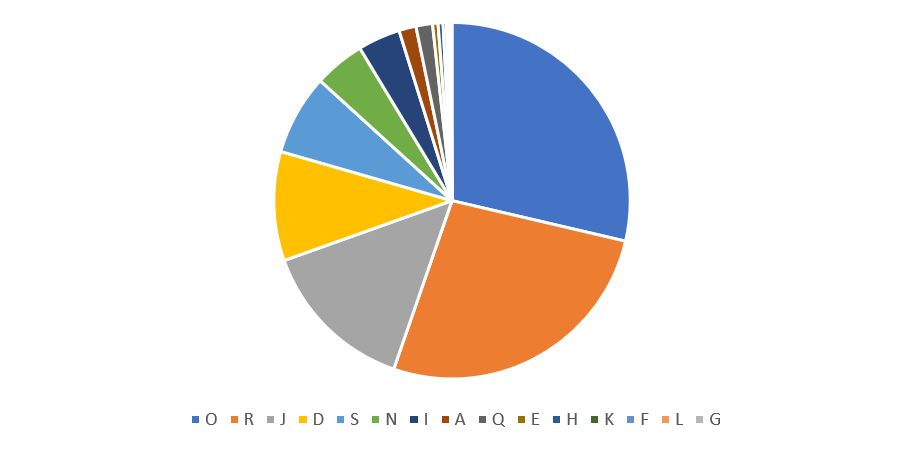
\includegraphics[width=0.8\textwidth]{Pie_Property_Info3.png}
	\end{center}
	\caption{Pie Graph Property\_Info3}
\end{figure}

\subsubsection{Property\_Info4}
\paragraph{Attribute type: nominal (dichotomous)}

\begin{table}[H]
	\renewcommand{\arraystretch}{1.25}
	\begin{tabular}{l|l}
		\textbf{Statistic} & \textbf{Value}\\\hline
		Missing Values& None\\\hline
	\end{tabular}
\end{table}
\begin{table}[H]
	\renewcommand{\arraystretch}{1.25}
	\begin{tabular}{l|l|l}
		\textbf{Value} & \textbf{Absolute Frequency} & \textbf{Relative Frequency}\\\hline
		1&$1364$&$0.682$\\\hline
		0&$636$&$0.318$
	\end{tabular}
\end{table}
\begin{figure}[H]
	\begin{center}
		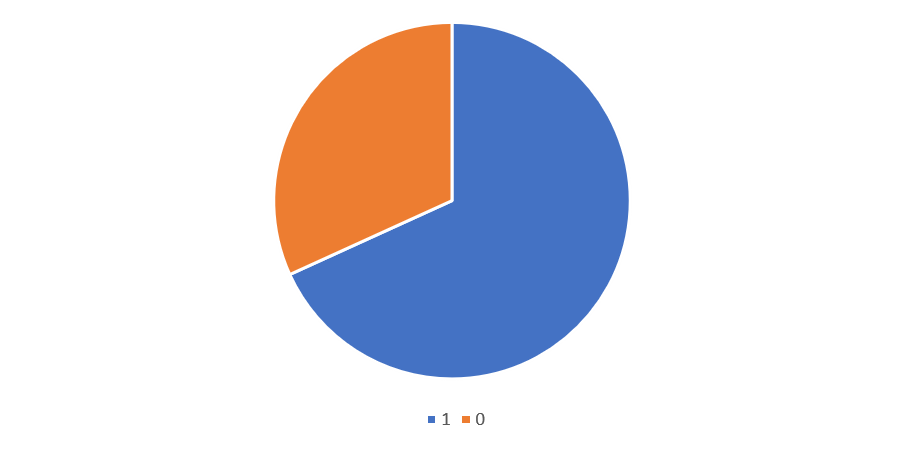
\includegraphics[width=0.8\textwidth]{Pie_Property_Info4.png}
	\end{center}
	\caption{Pie Graph Property\_Info4}
\end{figure}

\subsubsection{Property\_Info5}
\paragraph{Attribute type: ordinal} This Attribute too contains values from $1$ to $25$. I defined those as ordinal before.

\begin{table}[H]
	\renewcommand{\arraystretch}{1.25}
	\begin{tabular}{l|l}
		\textbf{Statistic} & \textbf{Value}\\\hline
		Missing Values& None\\\hline
	\end{tabular}
\end{table}

\begin{figure}[H]
	\begin{center}
		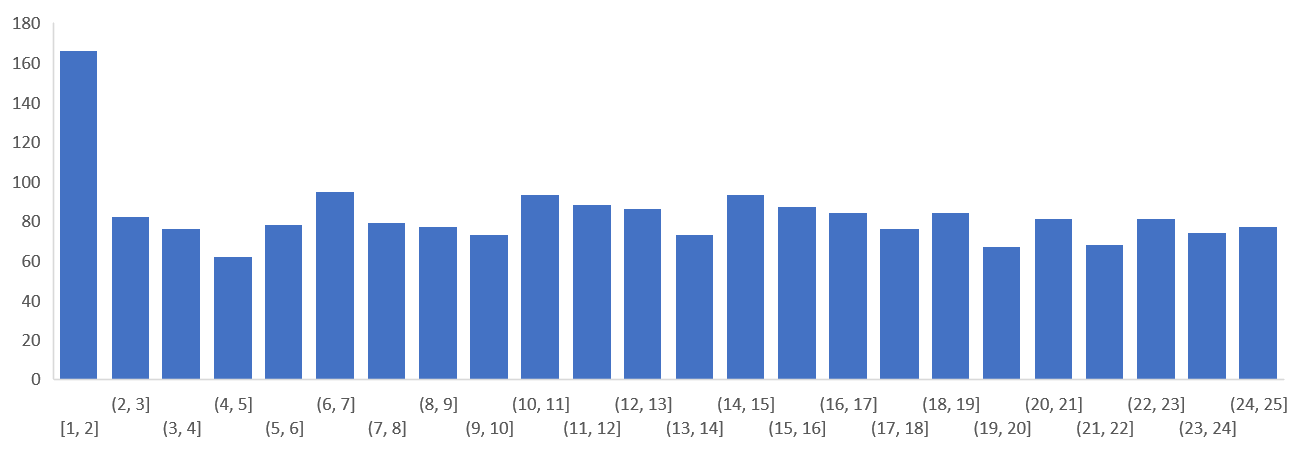
\includegraphics[width=0.8\textwidth]{Histo_Property_Info5.png}
	\end{center}
	\caption{Histogramm Property\_Info5}
\end{figure}

\subsubsection{Geographic\_Info1}
\paragraph{Attribute type: ordinal} This Attribute too contains values from $1$ to $25$. I defined those as ordinal before.

\begin{table}[H]
	\renewcommand{\arraystretch}{1.25}
	\begin{tabular}{l|l}
		\textbf{Statistic} & \textbf{Value}\\\hline
		Missing Values& None\\\hline
		Ouliers & 58
	\end{tabular}
\end{table}

\begin{figure}[H]
	\begin{center}
		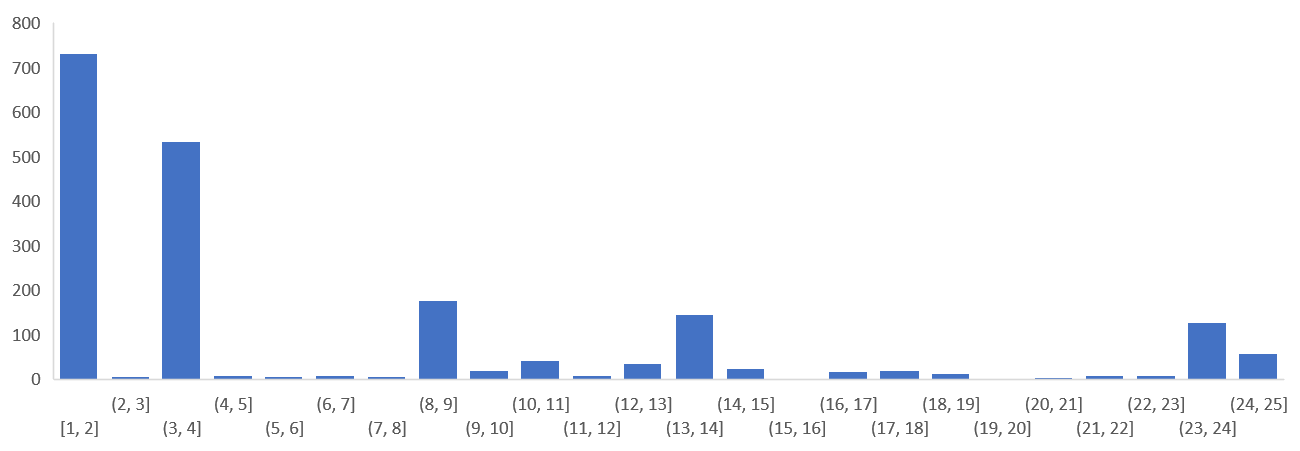
\includegraphics[width=0.8\textwidth]{Histo_Geographic_Info1.png}
	\end{center}
	\caption{Histogramm Geographic\_Info1}
\end{figure}

\subsubsection{Geographic\_Info2}
\paragraph{Attribute type: ordinal} This Attribute too contains values from $1$ to $25$. I defined those as ordinal before.

\begin{table}[H]
	\renewcommand{\arraystretch}{1.25}
	\begin{tabular}{l|l}
		\textbf{Statistic} & \textbf{Value}\\\hline
		Missing Values& None\\\hline		
	\end{tabular}
\end{table}

\begin{figure}[H]
	\begin{center}
		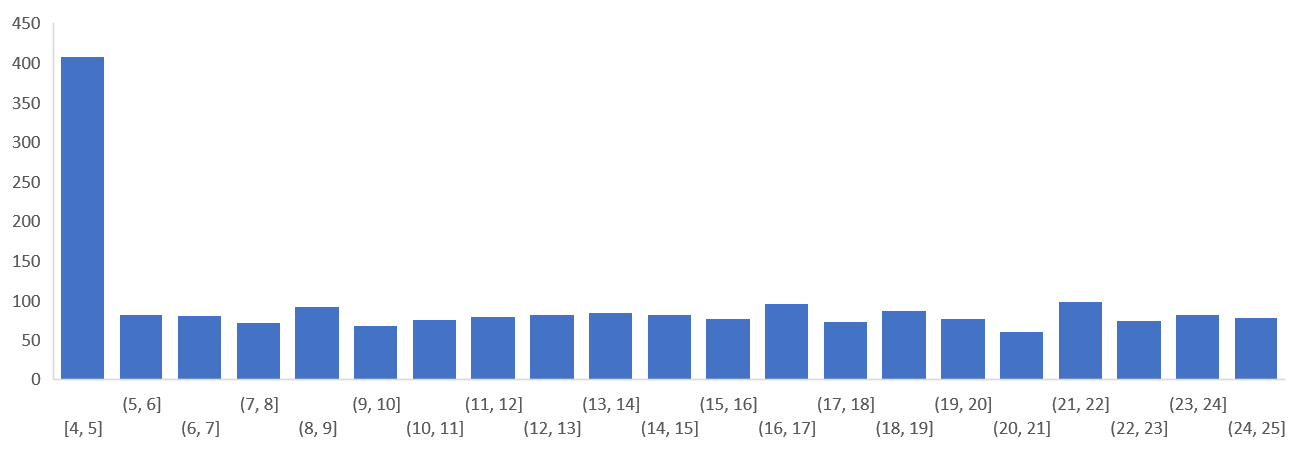
\includegraphics[width=0.8\textwidth]{Histo_Geographic_Info2.png}
	\end{center}
	\caption{Histogramm Geographic\_Info2}
\end{figure}

\subsubsection{Geographic\_Info3}
\paragraph{Attribute type: nominal} These values are very interessting. They could belong to a ordered attribute like "Personal\_Info2". Nevertheless, it is defined as nominal because too many values are missing.

\begin{table}[H]
	\renewcommand{\arraystretch}{1.25}
	\begin{tabular}{l|l}
		\textbf{Statistic} & \textbf{Value}\\\hline
		Missing Values& None\\\hline
	\end{tabular}
\end{table}
\begin{table}[H]
	\renewcommand{\arraystretch}{1.25}
	\begin{tabular}{l|l|l}
		\textbf{Value} & \textbf{Absolute Frequency} & \textbf{Relative Frequency}\\\hline
		-1&$1942$&$0.971$\\\hline
		25&$58$&$0.029$
	\end{tabular}
\end{table}

\subsubsection{Geographic\_Info4}
\paragraph{Attribute type: nominal (dichotomous)}\quad

\begin{table}[H]
	\renewcommand{\arraystretch}{1.25}
	\begin{tabular}{l|l}
		\textbf{Statistic} & \textbf{Value}\\\hline
		Missing Values& None\\\hline
	\end{tabular}
\end{table}
\begin{table}[H]
	\renewcommand{\arraystretch}{1.25}
	\begin{tabular}{l|l|l}
		\textbf{Value} & \textbf{Absolute Frequency} & \textbf{Relative Frequency}\\\hline
		N&$1961$&$0.9805$\\\hline
		Y&$39$&$0.0195$
	\end{tabular}
\end{table}
\begin{figure}[H]
	\begin{center}
		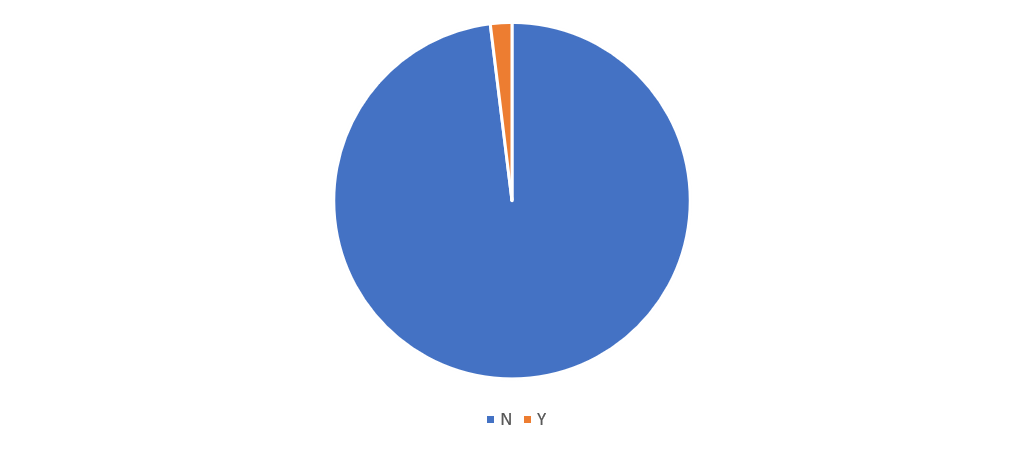
\includegraphics[width=0.8\textwidth]{Pie_Geographic_Info4.png}
	\end{center}
	\caption{Pie Graph Geographic\_Info4}
\end{figure}

\subsubsection{Geographic\_Info5}
\paragraph{Attribute type: nominal} These values could be the states California, New Jersey, Texas and Illinois. They also could represent any other value and don't have any specific order.

\begin{table}[H]
	\renewcommand{\arraystretch}{1.25}
	\begin{tabular}{l|l}
		\textbf{Statistic} & \textbf{Value}\\\hline
		Missing Values& None\\\hline
	\end{tabular}
\end{table}
\begin{table}[H]
	\renewcommand{\arraystretch}{1.25}
	\begin{tabular}{l|l|l}
		\textbf{Value} & \textbf{Absolute Frequency} & \textbf{Relative Frequency}\\\hline
		CA&$730$&$0.365$\\\hline
		NJ&$540$&$0.27$\\\hline
		TX&$491$&$0.2455$\\\hline
		IL&$239$&$0.1195$
	\end{tabular}
\end{table}

\begin{figure}[H]
	\begin{center}
		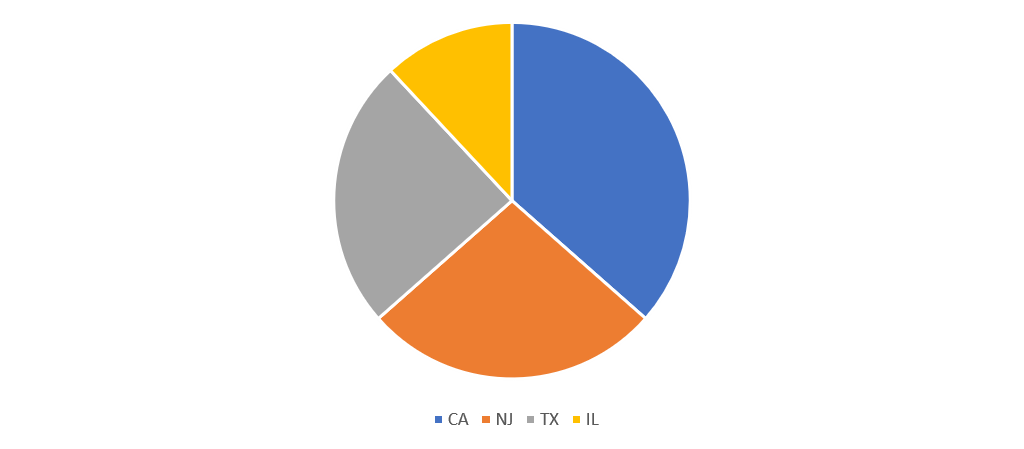
\includegraphics[width=0.8\textwidth]{Pie_Geographic_Info5.png}
	\end{center}
	\caption{Pie Graph Geographic\_Info5}
\end{figure}

\subsection{Data Exploration}

\subsubsection{Interresting Attribute Features}

\paragraph{Field\_Info3} All values in this attribute are either on the side or in the middle of the range. 

\paragraph{Field\_Info4} Normal distribution, but there is a peak at the end.

\paragraph{Coverage\_Info2} On this attribute we only have datapoints with four different values allthough the range of those values suggets 25 options have been available.

\paragraph{Geographic\_Info2 \& Property\_Info 5} Both of these values show a  even distribution with a spike at the begin of their ranges.

\paragraph{Personal\_Info3} Almost $50 \text{\%}$ of the values are "ZA".
\paragraph{Property\_Info2} All values are $0$
\paragraph{Personal\_Info4} All values are $0$ except for one $1$

\subsubsection{Linear Correlations}

There are some interesting correlations in this dataset. Especially Geographic\_Info5 seems to have some strong correlations with Field\_Info2 and Coverage\_Info3. Field\_Info1 seems to be correlated to Field\_Info4 and Field\_Info2 has as negative Correlation with Field\_Info3.

\begin{figure}[H]
	\begin{center}
		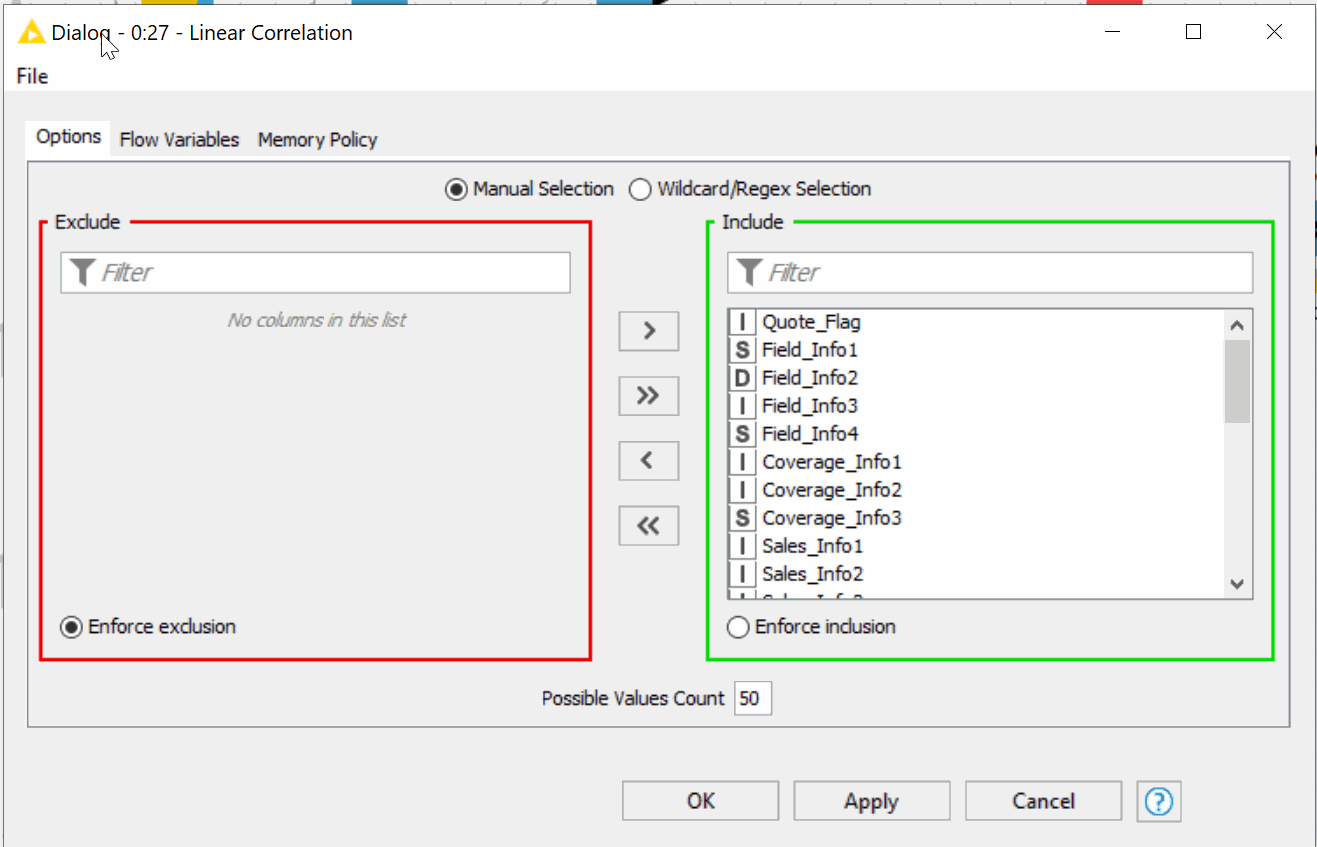
\includegraphics[width=0.4\textwidth]{Screen/Screen_Corr_1.png}
		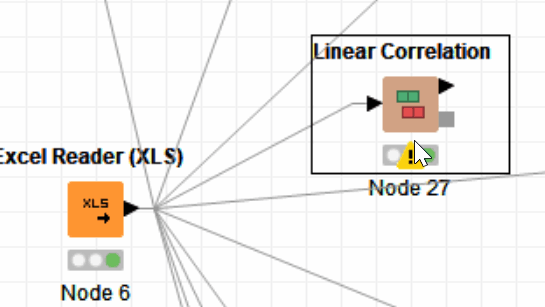
\includegraphics[width=0.4\textwidth]{Screen/Screen_Corr_3.png}
		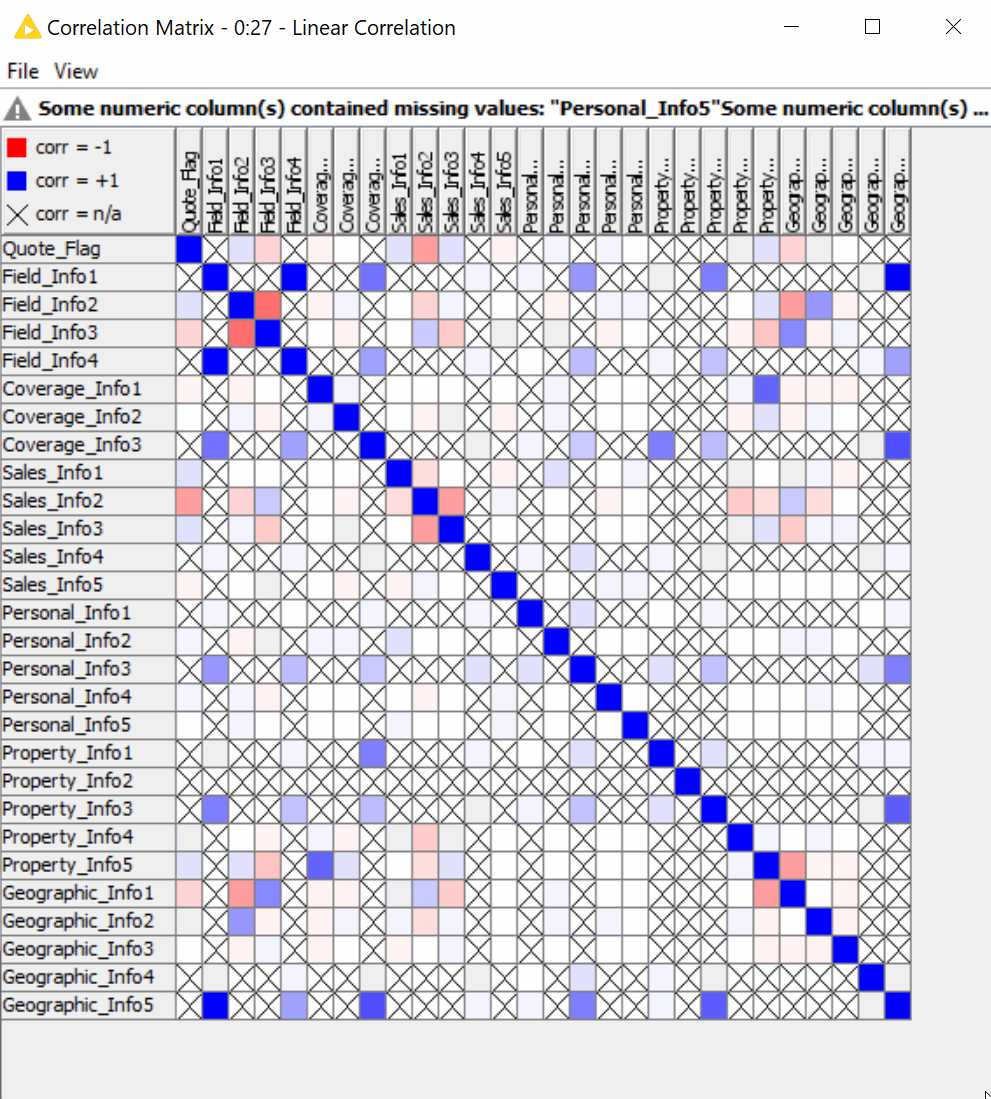
\includegraphics[width=0.4\textwidth]{Screen/Screen_Corr_2.png}

	\end{center}
	\caption{Screenshots Linear Correlation}
\end{figure}

\subsubsection{Patterns inside the data}

To find patterns inside the data I used KNIME and a local scatter plot linked with the color manager. This allowed me to find some interesting patterns and interrelations. In th following plots the colors are mapped to Geographic\_Info5.

Coverage\_Info1 and Property\_Info5 show a even distribution except for a part in the lower right corner of the plot, where no datapoint can be found if Property\_Info5 is greater than $12$ and Coverage\_Info lower than $7$.
\begin{figure}[H]
	\begin{center}
		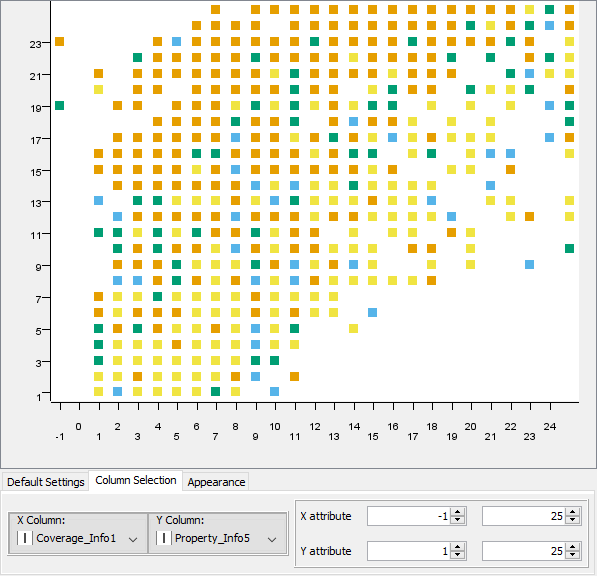
\includegraphics[width=0.4\textwidth]{Plots/Scatter_CI1-PI5.png}
	\end{center}
	\caption{Scatter Plot Coverage\_Info1 and Property\_Info5}
\end{figure}

If a dataset has the value B in Field\_Info2, its Field\_Info1 value will be between $910$ and $960$. Similar rules account for other values, too, as can be seen in the plot below.
\begin{figure}[H]
	\begin{center}
		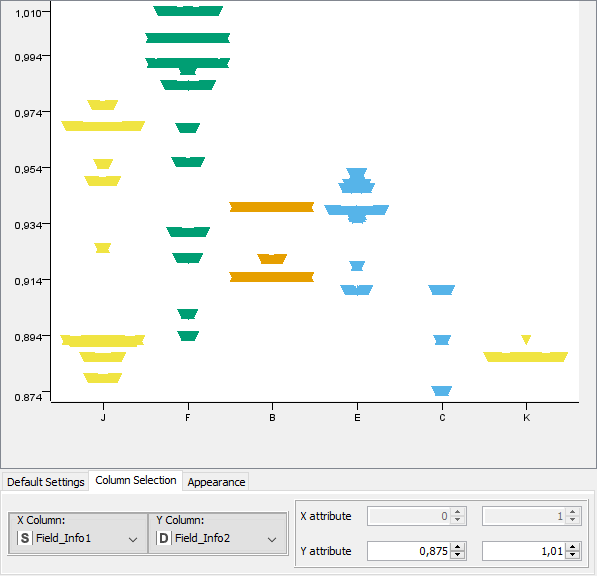
\includegraphics[width=0.4\textwidth]{Plots/Scatter_FI1-FI2.png}
	\end{center}
	\caption{Scatter Plot Field\_Info1 and Field\_Info2}
\end{figure}

A interessting grouping can be found with Field\_Info3 and Geographic\_Info2 where if Field\_Info3 is between $4$ and $16$, Geographic\_Info2 will be between $890$ and $1200$ and if it gets greater than $16$ most of Geographic\_Info2 will be at $548$ and at $1487$ when Field\_Info3 is greater than 22. 

\begin{figure}[H]
	\begin{center}
		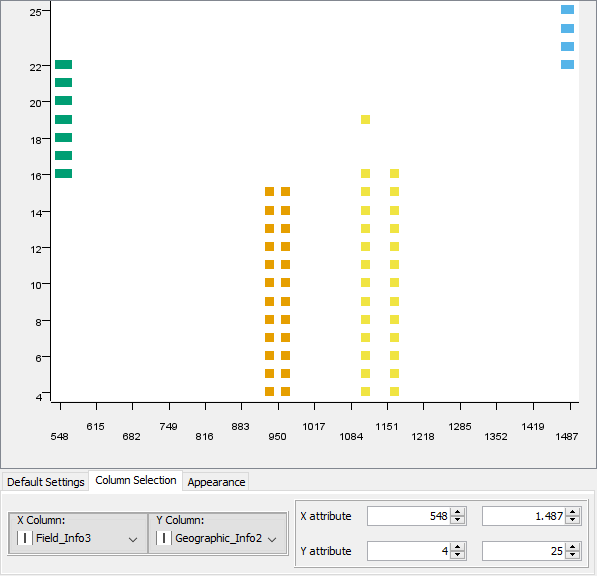
\includegraphics[width=0.4\textwidth]{Plots/Scatter_FI3-GI2.png}
	\end{center}
	\caption{Scatter Plot Field\_Info2 and Geographic\_Info2}
\end{figure}

Geographic\_Info5 has some interesting patterns with different other Attributes. The first one beeing Field\_Info4. If Geographic\_Info5 is "CA" or "NJ", Field\_Info4 will be "N". Another connection can be found to Field\_Info1 as can be seen below. 
\begin{figure}[H]
	\begin{center}
		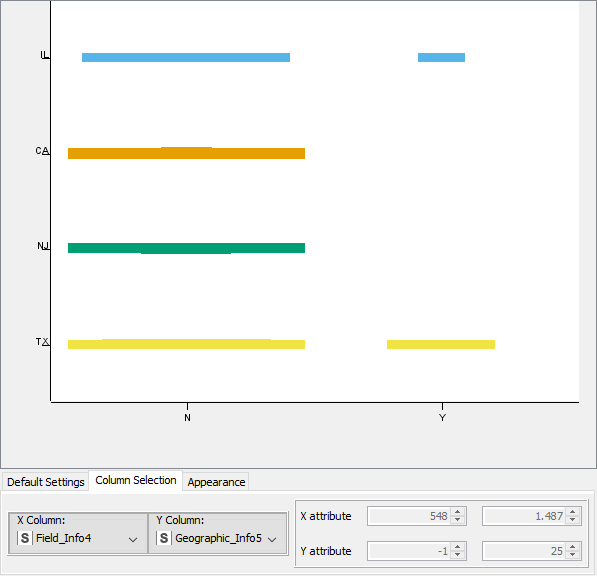
\includegraphics[width=0.4\textwidth]{Plots/Scatter_FI4-GI5.png}
	\end{center}
	\caption{Scatter Plot Field\_Info4 and Geographic\_Info5}
\end{figure}
\begin{figure}[H]
	\begin{center}
		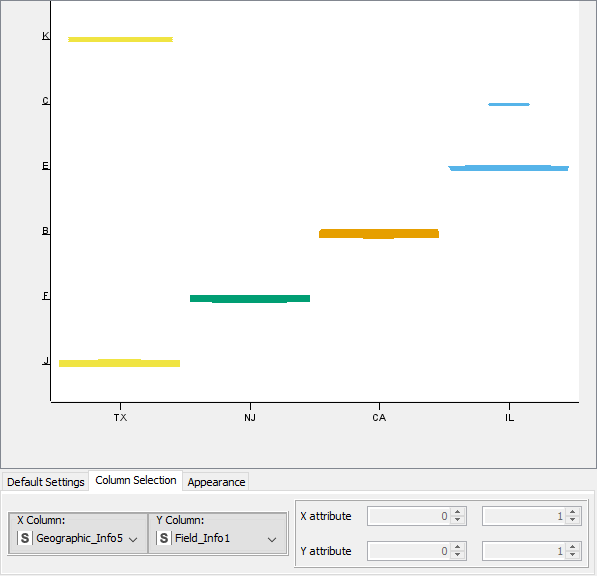
\includegraphics[width=0.4\textwidth]{Plots/Scatter_GI5-FI1.png}
	\end{center}
	\caption{Scatter Plot Geographic\_Info5 and Field\_Info5}
\end{figure}
\begin{figure}[H]
	\begin{center}
		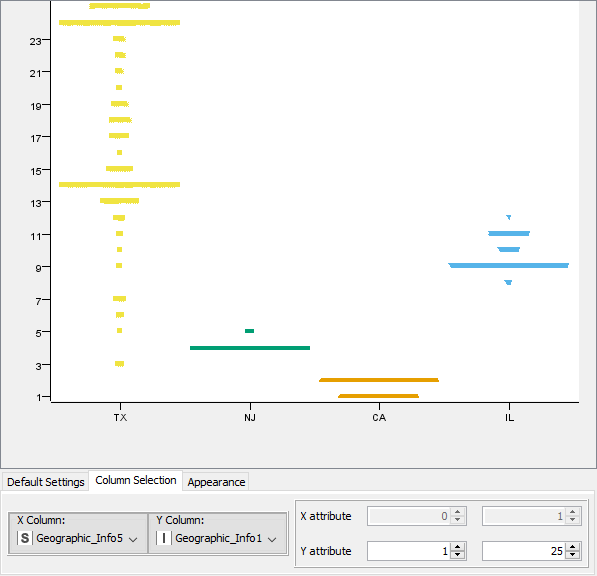
\includegraphics[width=0.4\textwidth]{Plots/Scatter_GI5-GI1.png}
	\end{center}
	\caption{Scatter Plot Geographic\_Info5 and Geographic\_Info1}
\end{figure}

A similar bahavior as between Field\_Info3 and Geographic\_Info2 can be found between Geographic\_Info5 and Geographic\_Info2.

\begin{figure}[H]
	\begin{center}
		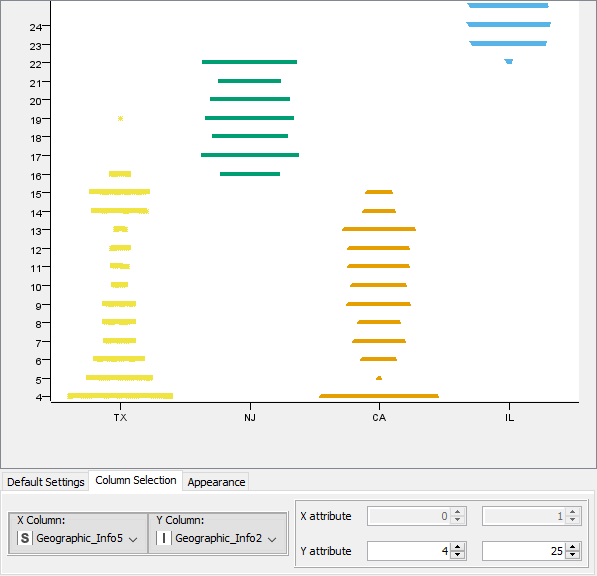
\includegraphics[width=0.4\textwidth]{Plots/Scatter_GI5-GI2.png}
	\end{center}
	\caption{Scatter Plot Geographic\_Info5 and Geographic\_Info2}
\end{figure}

Personal\_Info3 has some correlations with Geographic\_Info5 and Field\_Info1, where when Geographic\_Info5 is "CA", Personal\_Info3 is "B" and Field\_Info1 is "XW".

\begin{figure}[H]
	\begin{center}
		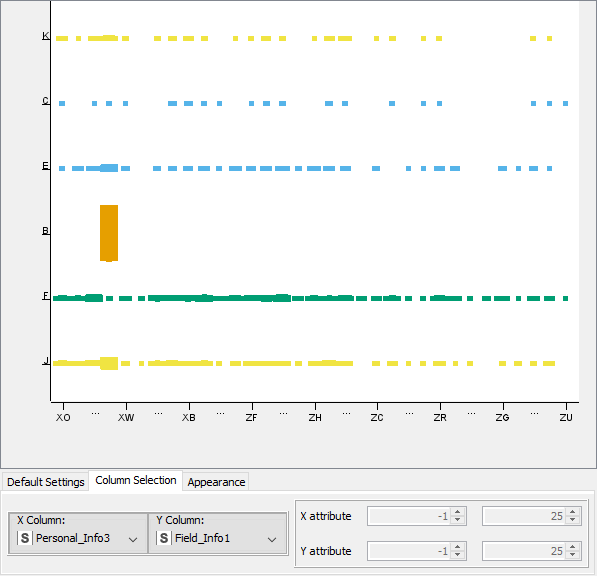
\includegraphics[width=0.4\textwidth]{Plots/Scatter_PI3-FI1.png}
	\end{center}
	\caption{Scatter Plot Geographic\_Info5 and Field\_Info1}
\end{figure}


\section{Data Preprocessing}
\subsection{Binning of Property\_Info5}	
To bin the different values of Property\_Info5 we have to decide how many bins we want to create. To do so we can use the following formula.
\begin{equation*}
k = \left \lceil \frac{\max x - \min x}{h} \right \rceil
\end{equation*}
Where $h$ is the Freedman–Diaconis rule:
\begin{equation*}
h=2\frac{\text{IQR}}{n^{1/3}}
\end{equation*}
Using this we can calculate the number of bins $k$ to be
\begin{align*}
\text{IQR} &= 19-7 = 12\\
n &= 2000\\
h&=2\frac{\text{IQR}}{n^{1/3}} = 2\frac{12}{2000^{1/3}} \approx 1.9\\
k&=\left \lceil \frac{\max x - \min x}{h} \right \rceil = \left \lceil \frac{25 - 1}{1.9} \right \rceil = 13
\end{align*}
With this number of bins, we can use Knime to bin our datapoints. The resulting binned data can be found inside of \texttt{data.xlsx}.
\begin{figure}[H]
	\begin{center}
		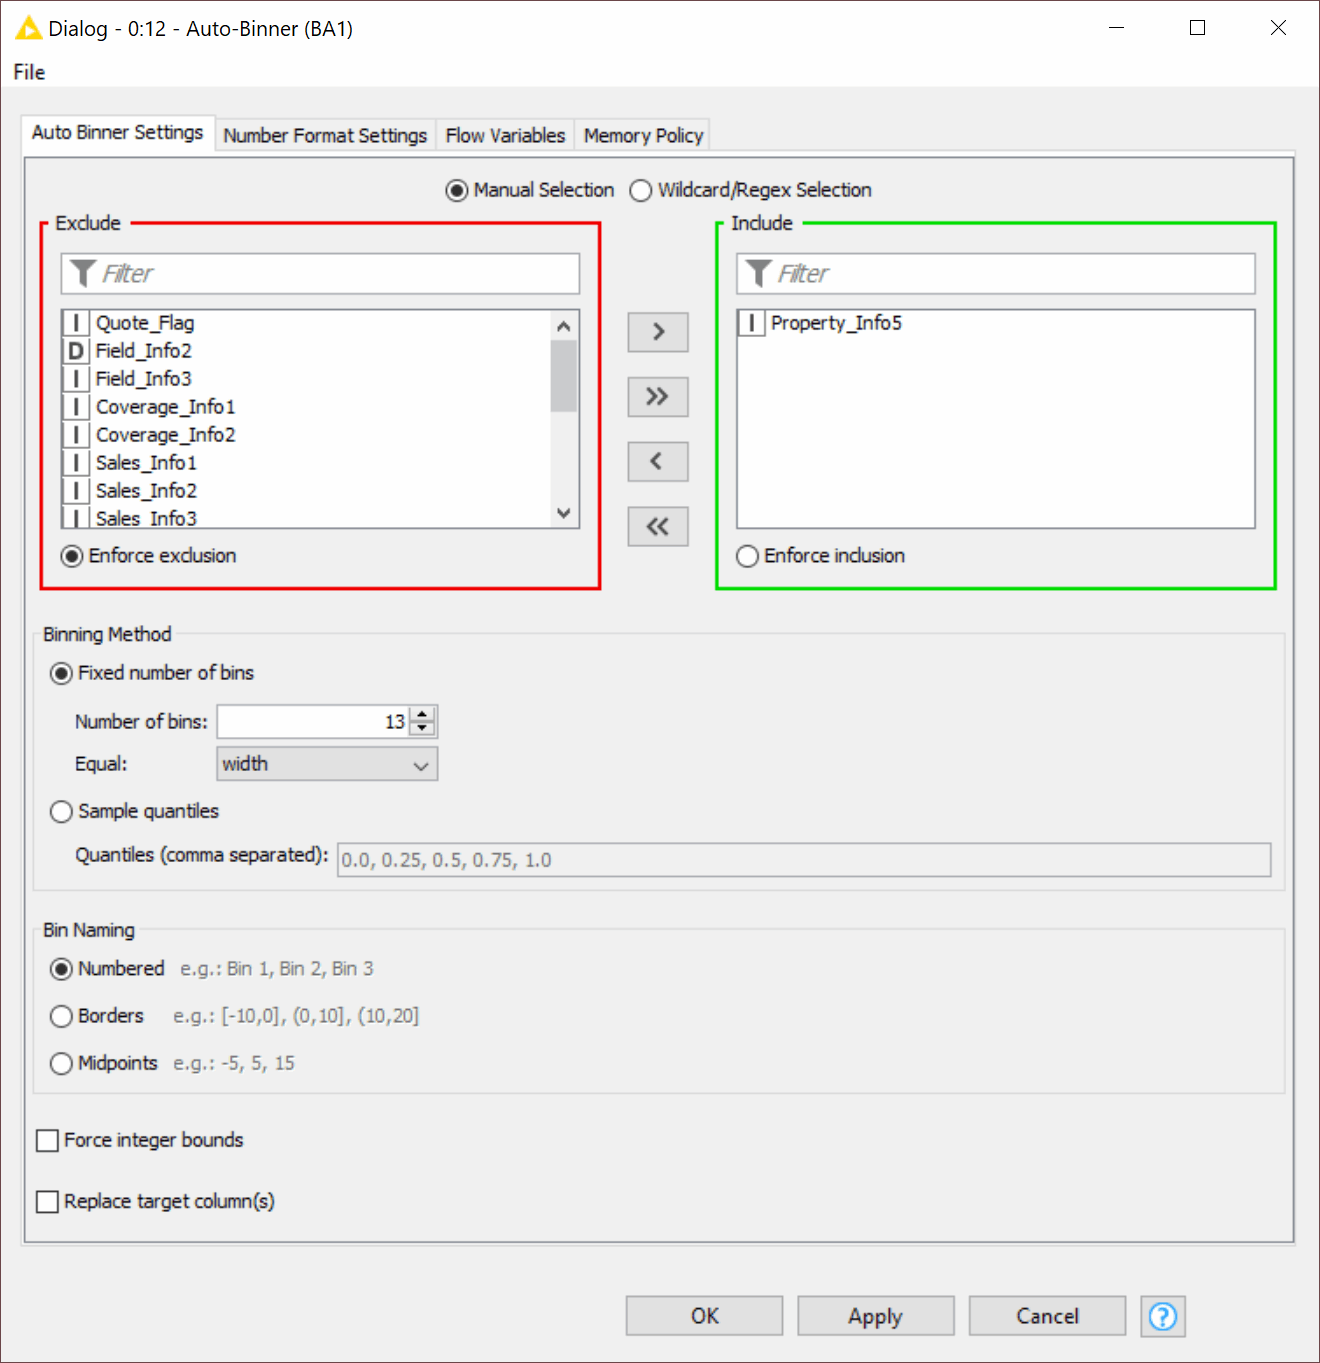
\includegraphics[width=0.4\textwidth]{Screen/Screen_Bin_1.png}
		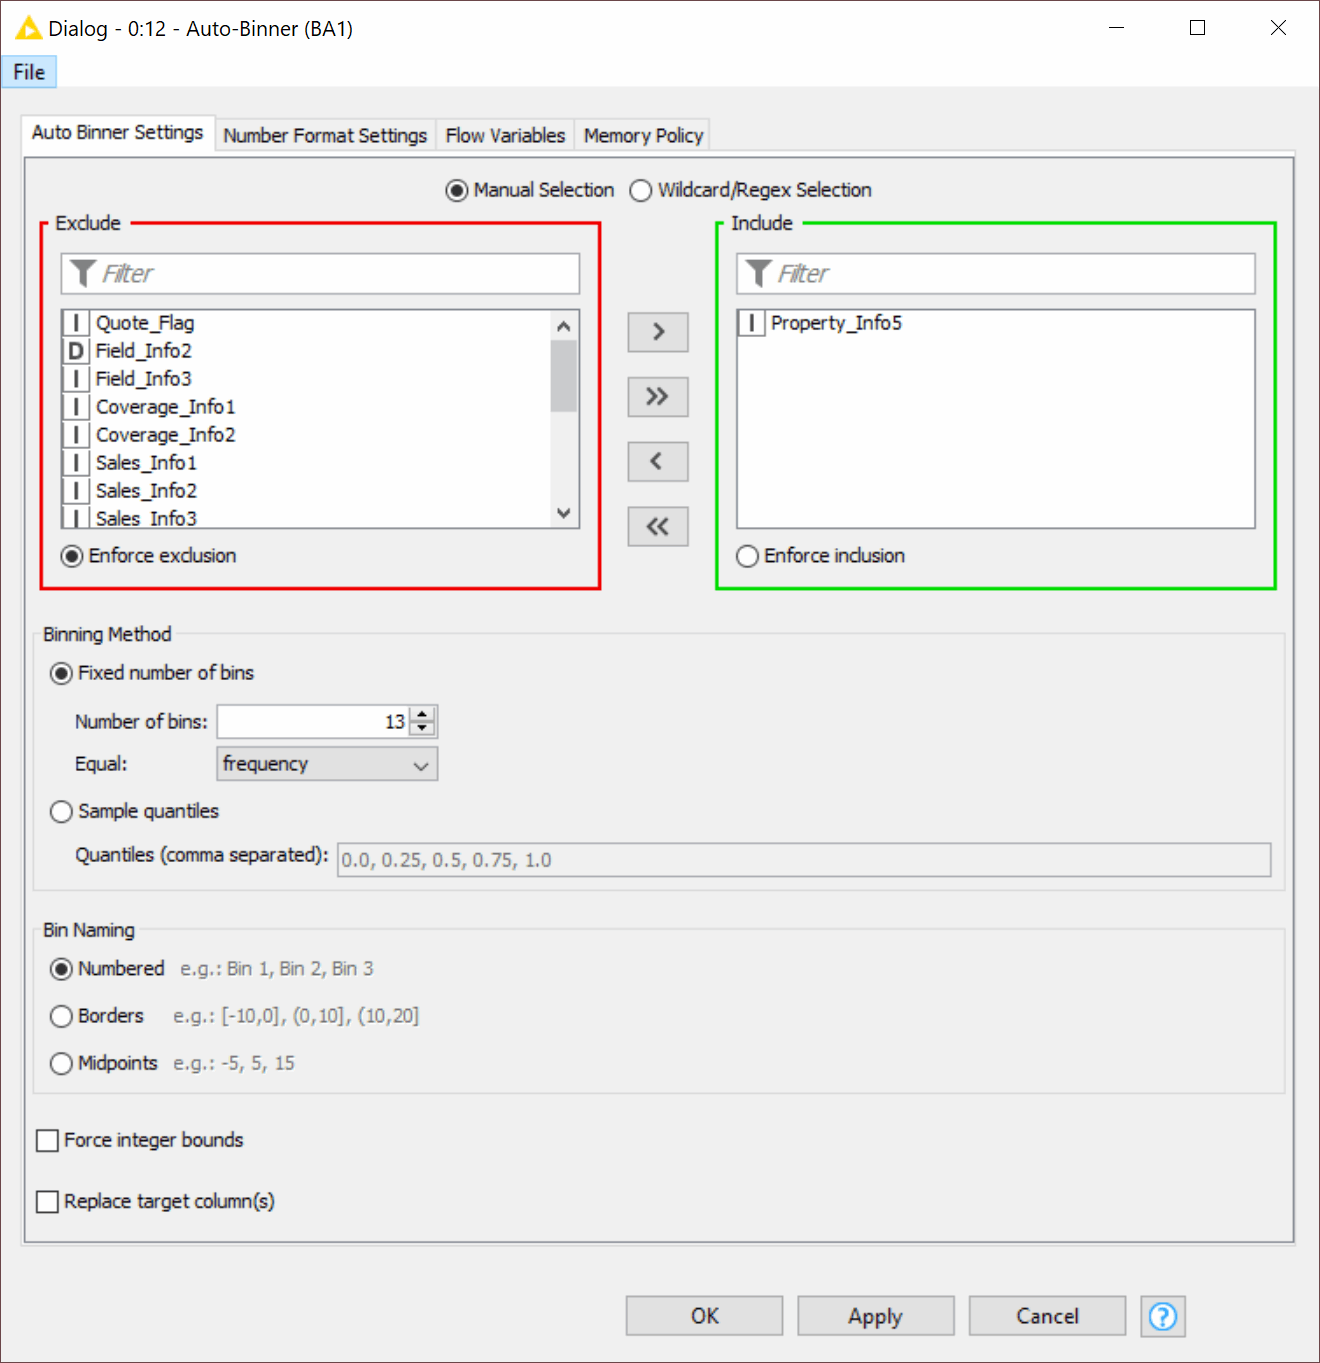
\includegraphics[width=0.4\textwidth]{Screen/Screen_Bin_2.png}
		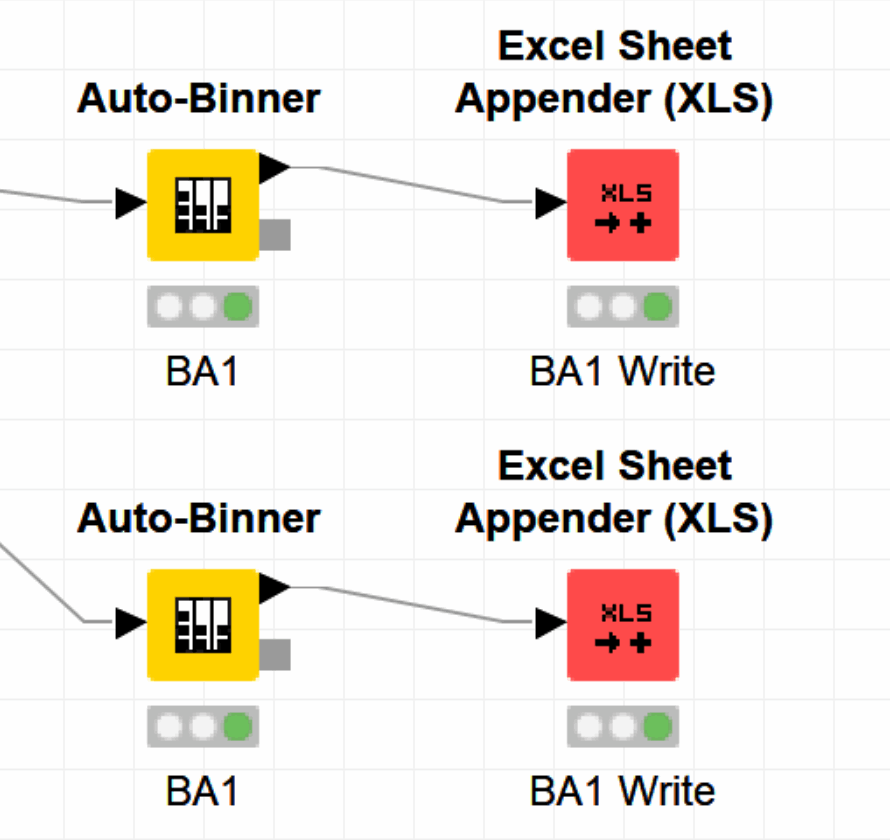
\includegraphics[width=0.4\textwidth]{Screen/Screen_Bin_3.png}
	\end{center}
	\caption{Screenshots Binning}
\end{figure}
\subsection{Normalization of Sales\_Info5}
Normalization describes a function to transfer values of different scales or of wide spread and undefinded borders into a common scale with defined endpoints. In this case we use min-max and z-scale normalization. Min-max will scale all values down to a range between $0$ and $1$ using the following formula:
\begin{equation*}
X'={\frac {X-X_{\min }}{X_{\max }-X_{\min }}}
\end{equation*}
The Z-Score normalization will remove ouliers inside a dataset. This will be done by using the following formula: 
\begin{equation*}
X'=\frac{X - \mu}{\sigma}
\end{equation*}
Where $\mu$ is the mean and $\sigma$ is the standard deviation.
\begin{figure}[H]
	\begin{center}
		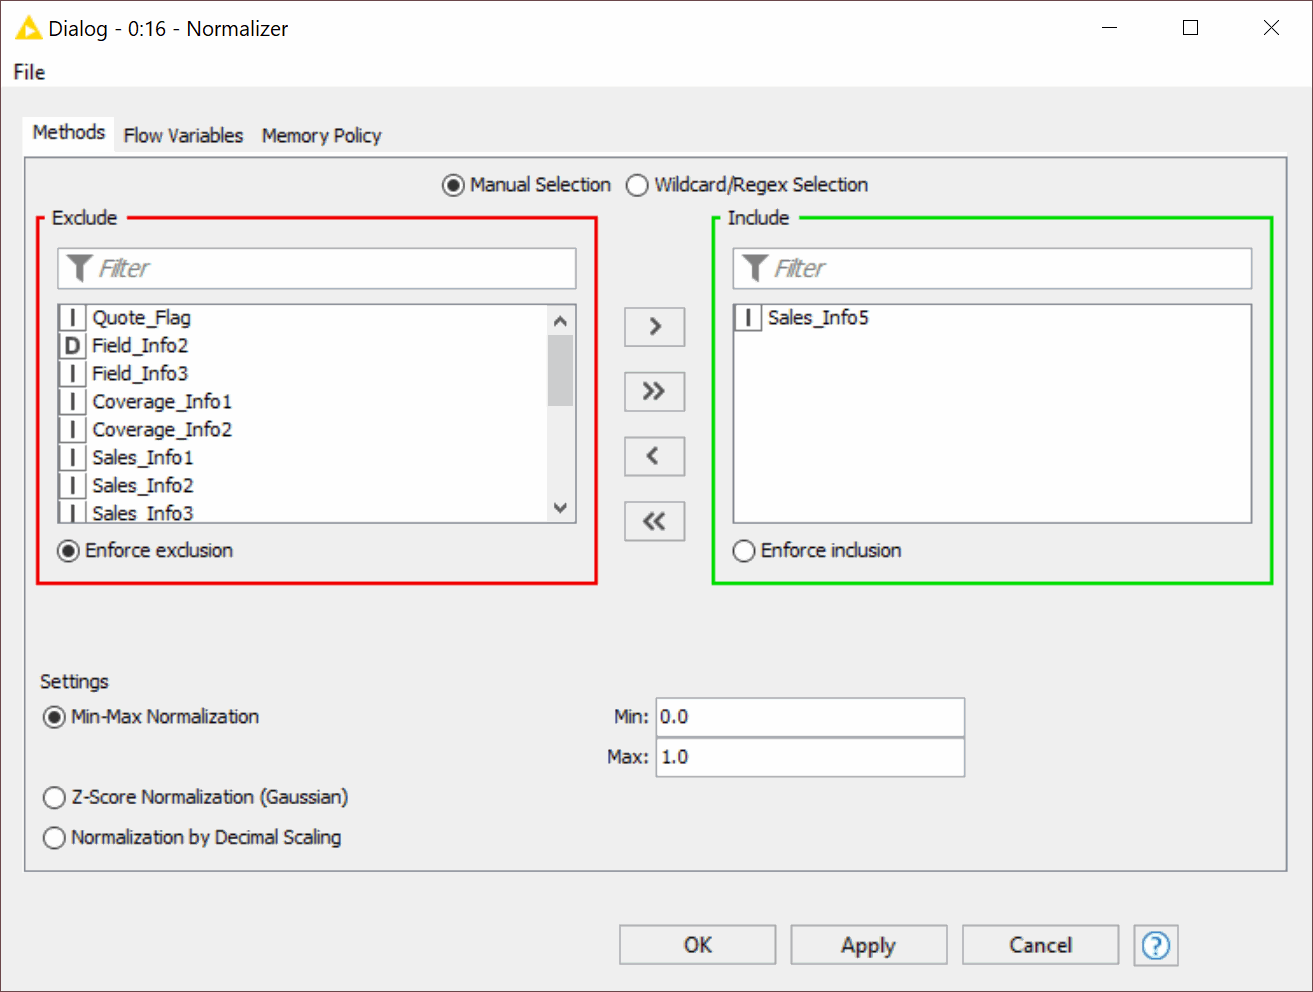
\includegraphics[width=0.4\textwidth]{Screen/Screen_Norm_1.png}
		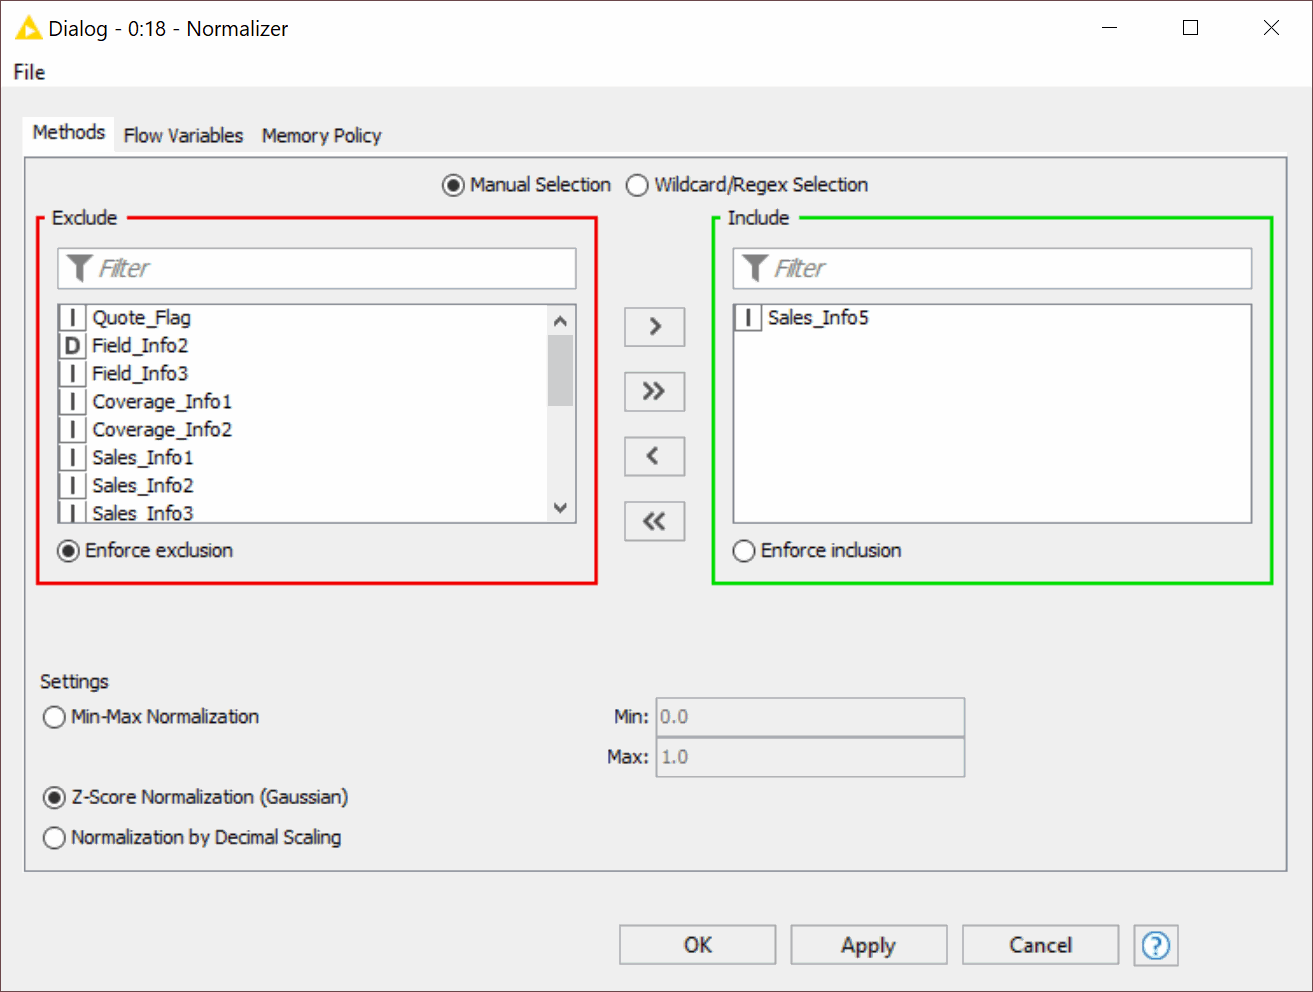
\includegraphics[width=0.4\textwidth]{Screen/Screen_Norm_2.png}
		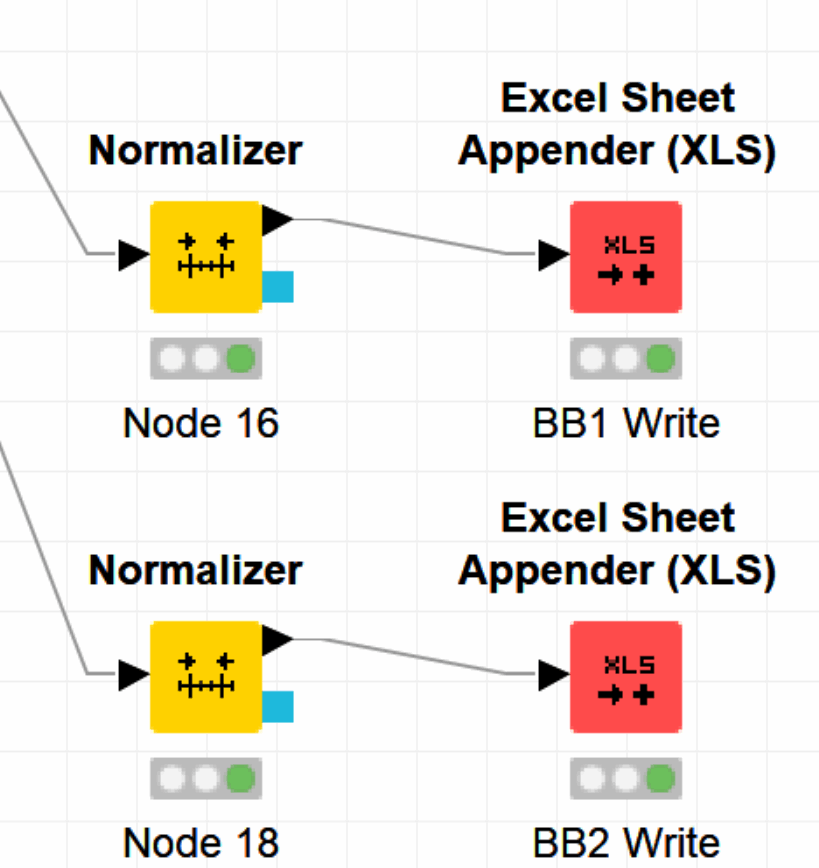
\includegraphics[width=0.4\textwidth]{Screen/Screen_Norm_3.png}
	\end{center}
	\caption{Screenshots Normalization}
\end{figure}
\subsection{Discretization of Coverage\_Info1}
Discretization is a process of transfering continous or wide spread values into discrete counterparts. In our case we will discretize by using equi-width binning.
 
Since the values in Coverage\_Info1 range from 1 to 25, it makes sense to set the range of each category to $6$ and the thresholds for the four categories as follows:
\begin{align*}
\text{Basic} &= ]-\infty , 7[ & 763\quad\text{elements}\\
\text{Low} &= ]7 , 13[& 786\quad\text{elements}\\
\text{Medium} &= ]13 , 19[& 303\quad\text{elements}\\
\text{High} &= ]19 , \infty[& 148\quad\text{elements}
\end{align*}
\begin{figure}[H]
	\begin{center}
		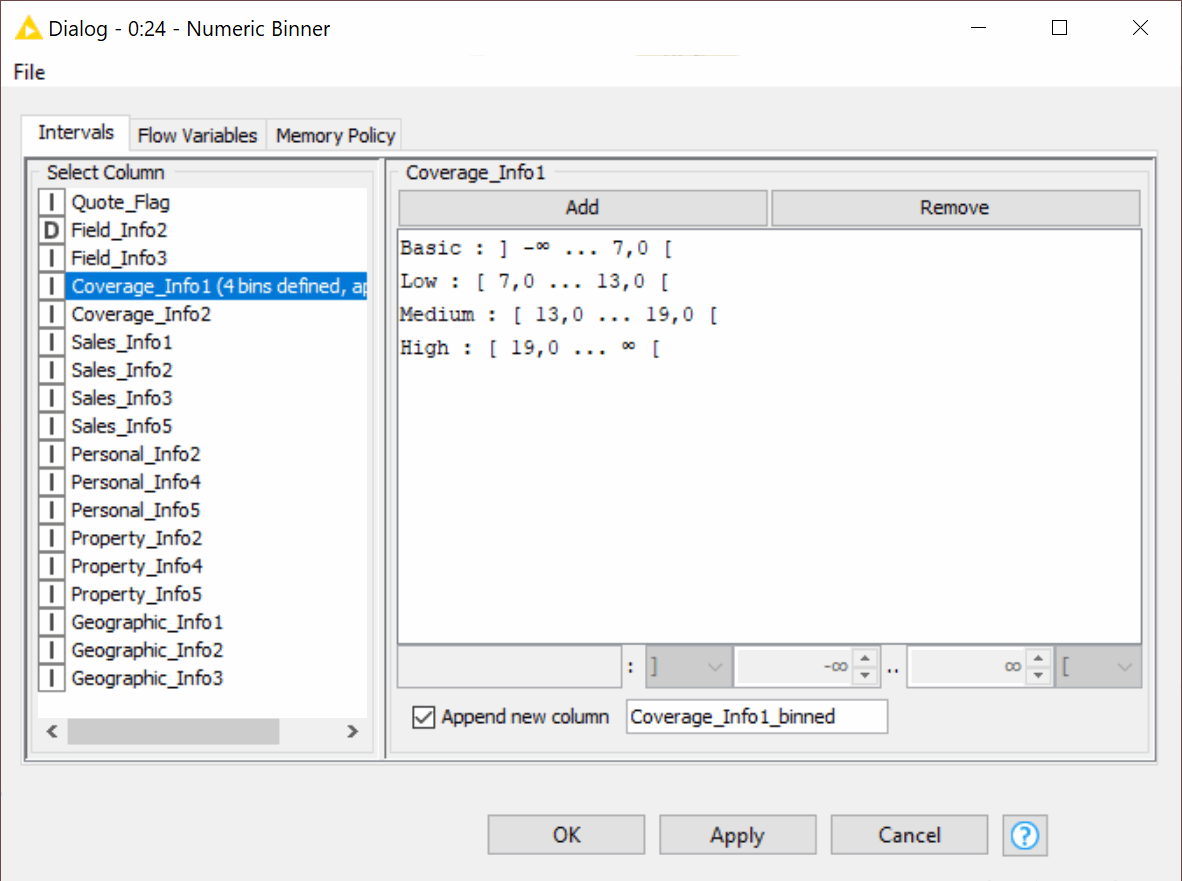
\includegraphics[width=0.8\textwidth]{Screen/Screen_Num_1.png}
		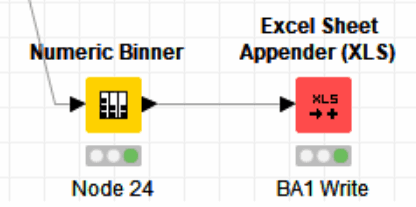
\includegraphics[width=0.5\textwidth]{Screen/Screen_Num_2.png}	
	\end{center}
	\caption{Screenshots Discretization}
\end{figure}
\subsection{Binarization of Geographic\_Info5}
Binarization is a transformation of data features from single attributes into binary vectors. This spreads out one nominal attribute into multiple binary attributes. This process can make classifier algorithms more efficient.

To binarise the Attribute I used the "One to Many" Node in Knime. The result of the binarization can be found inside the attached excel-workbook.
\begin{figure}[H]
	\begin{center}
		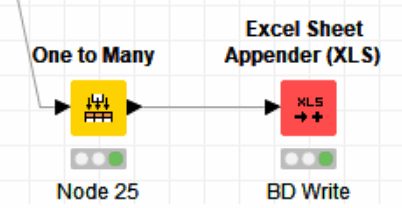
\includegraphics[width=0.4\textwidth]{Screen/Screen_Bina_1.png}
		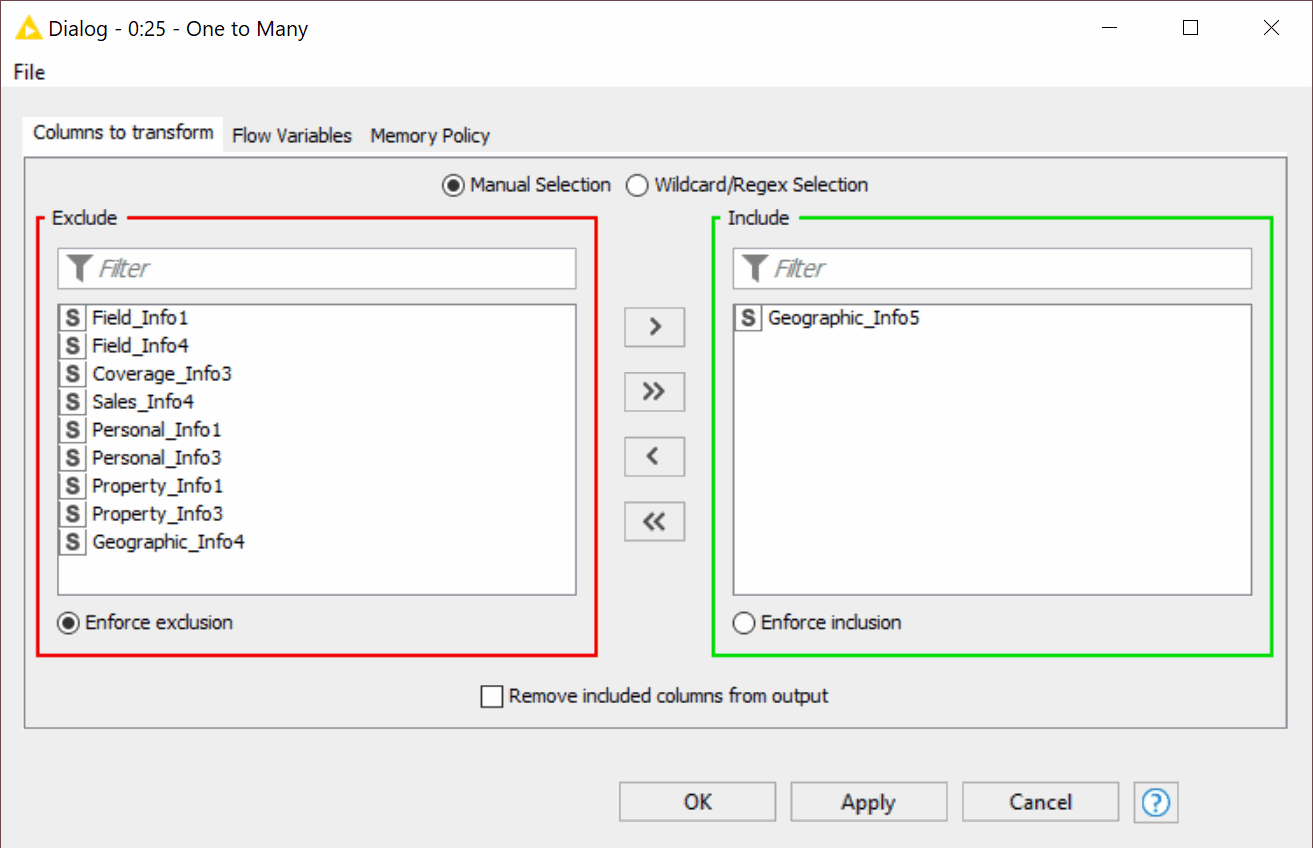
\includegraphics[width=0.4\textwidth]{Screen/Screen_Bina_2.png}
		
	\end{center}
	\caption{Screenshots Binarization}
\end{figure}
\pagebreak
\section{Summary}

During the exploration of the given data I was able to divide the results into three different sections.
The first of these sections are the peculiarities of the existing data points or their attributes.\\
With the attributes I could determine some interesting points. Some attributes had large shares of a value. This includes Property\_Info2, where only the value $0$ occurred. Also Personal\_Info4 has only the value $0$ except for one exception which has the value $1$. This is either a data error or an outlier. The attribute Personal\_Info3 is assigned the value "ZA" to almost $50$ %.\\
Field\_Info3 has an interesting value distribution, since all values are either at the outer edges or in the middle of the value range.\\
With Field\_Info4 a normal distribution of the values can be observed. The only exception to this is the largest value, which stands out due to a strong increase.\\
On this Coverage\_Info2 we only have data points with four different values although the range of those values suggest 25 options have been available.\\
Both, Geographic\_Info2 and Property\_Info5 show a even distribution, but both have a peak at the begin of their ranges, double the volume then the following values.

Some of the provided attributes show a linear correlation to each other.\\ Especially Geographic\_Info5 seems to have a strong correlation with Field\_Info2 and Coverage\_Info3. Field\_Info1 seems to be correlated to Field\_Info4 and Field\_Info2 has as negative Correlation with Field\_Info3.

When I did a cross comparison for some attributes, I was able to find some interesting patterns. Very interesting for future sales could be the connection between geographic information and other information as the Geographic\_Info5 has a lot of connection to different other attributes, sometimes even excluding specific values for other attributes. Also the attribute Personal\_Info3 has a correlation with Field\_Info1 and Geographic\_Info5.










% Verzeichnisse
\clearpage
\listoffigures
%\cleardoublepage

\listoftables
%\cleardoublepage

%\lstlistoflistings
%\cleardoublepage

%\newcommand{\abkvz}{Abkürzungsverzeichnis}
%\renewcommand{\nomname}{\abkvz}
%\section*{\abkvz}
%\markboth{\abkvz}{\abkvz}
%\addcontentsline{toc}{section}{\abkvz}
%% !TEX root = Ausarbeitung.tex

% Es werden nur die Abkürzungen aufgelistet, die mit \ac definiert und auch benutzt wurden. 
%
% \acro{VERSIS}{Versicherungsinformationssystem\acroextra{ (Bestandsführungssystem)}}
% Ergibt in der Liste: VERSIS Versicherungsinformationssystem (Bestandsführungssystem)
% Im Text aber: \ac{VERSIS} -> Versicherungsinformationssystem (VERSIS)

% Hinweis: allgemein bekannte Abkürzungen wie z.B. bzw. u.a. müssen nicht ins Abkürzungsverzeichnis aufgenommen werden
% Hinweis: allgemein bekannte IT-Begriffe wie Datenbank oder Programmiersprache müssen nicht erläutert werden,
%          aber ggfs. Fachbegriffe aus der Domäne des Prüflings (z.B. Versicherung)

% Die Option (in den eckigen Klammern) enthält das längste Label oder
% einen Platzhalter der die Breite der linken Spalte bestimmt.
\begin{acronym}[WWWWW]
	\acro{API}{Application Programming Interface}
	\acro{CI}{Continous Integration}
	\acro{IDE}{Integrated Development Environment}
	\acro{SDK}{Software Development Kit}
	\acro{SaSS}{Software as a Service}
    \acro{UI}{Benutzeroberfläche (engl.: "`User Interface"')}
    \acro{VCS}{Version Control System}
    \acro{CI}{Kontinuierliche Integration (engl.: "Continuous Integration")}
    \acro{VM}{Virtuelle Maschine}
    \acro{CPU}{Central Processing Unit}
    \acro{SPARC}{Scalable Processor ARChitecture}
    \acro{LXC}{Linux Containers}
    \acro{OCI}{Open Container Initiative}
\end{acronym}


% Literatur ------------------------------------------------------------------

%\renewcommand{\refname}{Literaturverzeichnis}
%\bibliography{Bibliographie}
%\bibliographystyle{Allgemein/natdin} % DIN-Stil des Literaturverzeichnisses
%\bibliographystyle{alphadin}
%% !TEX root = Projektdokumentation.tex
\clearpage
\addsec{Eidesstattliche Erklärung}

% Hinweis: die eidesstattliche Erklärung ist ggfs. an die Richtlinie der IHK anzupassen

Ich, \autorName, versichere hiermit, dass ich meine \textbf{\betreff} mit dem
Thema
\begin{quote}
\textit{\kompletterTitel}
\end{quote}
selbständig verfasst und keine anderen als die angegebenen Quellen und Hilfsmittel benutzt habe,
wobei ich alle wörtlichen und sinngemäßen Zitate als solche gekennzeichnet habe. Die Arbeit
wurde bisher keiner anderen Prüfungsbehörde vorgelegt und auch nicht veröffentlicht.\\[6ex]

\abgabeOrt, den \abgabeTermin


\rule[-0.2cm]{5.5cm}{0.5pt}

\textsc{\autorName}
 % Eidesstattliche Erklärung nur wenn von nöten drucken

% Anhang ---------------------------------------------------------------------
%\clearpage
%\appendix
%\pagenumbering{Roman}
%% !TEX root = Ausarbeitung.tex
\section{Anhang}
\label{sec:anhang}





\end{document}
